\documentclass[11pt]{elsarticle}


%% --------------------------------------------------------
%%  Packages
%% --------------------------------------------------------
\usepackage{xcolor}
\usepackage[colorlinks=true,linkcolor=blue,citecolor=red]{hyperref}
\usepackage{amsmath,amssymb,amsthm}
\usepackage{esint}
\usepackage{enumitem}
\usepackage{mathrsfs}
\usepackage{tikz}
\usetikzlibrary{arrows.meta, positioning, decorations.pathreplacing, calc}
\usepackage{booktabs}
\usepackage{graphicx}

%% --------------------------------------------------------
%%  Enumeration style
%% --------------------------------------------------------
\setenumerate{label=(\alph*)}
\setenumerate[2]{label=(\Alph*)}

%% --------------------------------------------------------
%%  Theorem environments (numbered within sections)
%% --------------------------------------------------------
\newtheorem{theorem}{Theorem}[section]
\newtheorem{proposition}[theorem]{Proposition}
\newtheorem{lemma}[theorem]{Lemma}
\newtheorem{corollary}[theorem]{Corollary}

\theoremstyle{definition}
\newtheorem{definition}[theorem]{Definition}
\newtheorem{example}[theorem]{Example}

\theoremstyle{remark}
\newtheorem{remark}[theorem]{Remark}

\numberwithin{equation}{section}

%% --------------------------------------------------------
%%  Math operators
%% --------------------------------------------------------
\def\diam{\operatorname{diam}}
\def\dist{\operatorname{dist}}
\def\supp{\operatorname{supp}}
\def\Ker{\operatorname{Ker}}
\def\Im{\operatorname{Im}}
\def\loc{\operatorname{loc}}
\def\gr{\operatorname{gr}}
\DeclareMathOperator*{\esssup}{ess\,sup}
\DeclareMathOperator*{\essinf}{ess\,inf}
\DeclareMathOperator{\argmin}{argmin}
\DeclareMathOperator{\Sign}{Sign}

%% --------------------------------------------------------

\setcounter{tocdepth}{2}% to get subsubsections in toc

\let\oldtocsection=\tocsection

\let\oldtocsubsection=\tocsubsection

\let\oldtocsubsubsection=\tocsubsubsection

\newcommand{\tocsection}[2]{\hspace{0em}\oldtocsection{#1}{#2}\textbf}
\newcommand{\tocsubsection}[2]{\hspace{1em}\oldtocsubsection{#1}{#2}}
\newcommand{\tocsubsubsection}[2]{\hspace{2em}\oldtocsubsubsection{#1}{#2}}

\begin{document}
	
	\begin{frontmatter}
		
		\title{Distance-Residual Physics-Informed Neural Networks:\\
			A Deep Learning Framework for Differential and\\
			Partial Differential Inclusions}
		
		\author[verkin]{Maria Filipkovska}
		\author[upct]{Juan Jos\'e Mar\'{\i}n}
		\author[itu]{Isil Oner}
		\author[upct]{Francisco Periago\corref{cor}}
		\author[coper]{Krzysztof Rykaczewski}
		
		\cortext[cor]{Corresponding author}
		
		\address[verkin]{B.\,Verkin Institute for Low Temperature Physics and Engineering of the National Academy of Sciences of Ukraine,
			Kharkiv 61103, Ukraine.}
		
		\address[upct]{Department of Applied Mathematics and Statistics,
			Universidad Polit\'ecnica de Cartagena, member of the European University of Technology EUT+,
			Campus Muralla del Mar, 30202 Cartagena, Murcia, Spain.}
		
		\address[itu]{Department of Mathematics, Faculty of Sciences,
			Gebze Technical University, Kocaeli 41400, Turkey.}
		
		\address[coper]{Faculty of Mathematics and Computer Science, Nicolaus Copernicus University, Chopina 12/18, 87-100
			Torun, Poland}
		
		\begin{abstract}
			We introduce \emph{Distance-Residual Physics-Informed Neural Networks}
			(DR-PINNs), a supervised learning framework for approximating solutions
			of differential and partial differential inclusions --- governing laws in
			which a differential operator is constrained to lie in a set-valued map
			rather than equaling a prescribed function.  The central idea is a single
			unifying principle: replace the classical pointwise PDE/ODE residual by
			the squared distance from the differential operator to the admissible set.
			This substitution is natural (the distance vanishes precisely when the
			inclusion is satisfied), geometrically interpretable (it measures the
			minimum correction needed for the operator to enter the admissible set),
			and amenable to gradient-based training: for a fixed closed convex
			admissible set, the squared distance is differentiable with respect to
			the operator value, with gradient given by the metric projection. When
			the admissible set also depends on the network state, that dependence
			must additionally be included by the chain rule.
			The framework encompasses ordinary differential inclusions and 
			partial differential inclusions with set-valued reaction terms.
			For both settings we prove \emph{consistency}:
			any sequence of network approximations whose distance residual converges
			to zero must converge, along a subsequence, to an exact solution of the
			target inclusion.  The proofs combine a priori estimates (Gr\"onwall
			inequality and parabolic energy estimates), weak compactness arguments
			(Arzel\`a--Ascoli and Aubin--Lions), and the lower semicontinuity of
			normal convex integrands.  For admissible sets given as convex hulls of
			finitely many vertices, projection onto the set reduces to a small convex
			quadratic program, making the loss efficiently computable inside the
			training loop.  Numerical experiments on benchmark differential
			inclusions and parabolic inclusions demonstrate the accuracy and
			flexibility of DR-PINNs.
		\end{abstract}
		
		\begin{keyword}
			Physics-Informed Neural Networks \sep
			distance function \sep
			differential inclusions \sep
			partial differential inclusions  \sep
			consistency analysis.
			\MSC[2020] 34A60 \sep 49J53 \sep 65M99 \sep 68T07.
		\end{keyword}
		
	\end{frontmatter}
	
	\tableofcontents
	\newpage
	
	%% ============================================================
	\section{Introduction}
	\label{sec:intro}
	%% ============================================================
	
	Physics-Informed Neural Networks (PINNs) have emerged as a powerful
	paradigm for approximating solutions of differential equations by
	embedding the governing physical laws directly into the training loss
	\cite{raissi2019}.  Since the foundational work of Raissi, Perdikaris,
	and Karniadakis, the PINN framework has been applied to a broad spectrum
	of problems: nonlinear partial differential equations (PDEs) in fluid
	mechanics, heat transfer, and wave propagation; inverse problems and
	parameter identification; operator learning; and high-dimensional
	stochastic differential equations.  The approach shares a common
	structural feature across all of these applications: the governing law
	takes the form of an equality, either an ordinary differential equation
	(ODE) of the form $\dot{x}(t) = f(t,x(t))$ or a PDE of the form
	$\mathcal{D}(u) = f$, and the PINN loss is built from the \emph{pointwise
		residual} obtained by substituting a neural-network surrogate into that
	equality.
	
	A class of mathematical models which does not fit within this
	framework is the one whose governing law takes the \emph{set-valued} form
%	In many applications --- control theory and optimal control
%	\cite{aubin_cellina_1984}, mechanics of systems with unilateral
%	constraints \cite{deimling_1992}, nonsmooth dynamics, phase-field models
%	with discontinuous constitutive laws, reaction-diffusion systems with
%	uncertain or multivalued kinetics, and multivalued variational problems
%	--- 
	\[
	\mathcal{D}(u) \in \mathcal{F}(u),
	\]
	where $\mathcal{F}(u)$ is a multifunction (set-valued map).  Concrete
	instances include:
	\begin{itemize}
		\item \emph{Differential inclusions}: $\dot{x}(t)\in F(t,x(t))$,
		where $F(t,x)$ is a set of admissible velocities;
		\item \emph{Parabolic partial differential inclusions}:
		$\partial_t u - \Delta u \in \Phi(u)$, where $\Phi(u)$ is a
		set-valued reaction term.
	\end{itemize}
	In all of these cases the classical notion of residual breaks down,
	because there is no single-valued right-hand side against which the
	differential operator can be compared. 	
	A simple geometric observation to overcome this difficulty is the following.  Given any
	set-valued law $\mathcal{D}(u)\in\mathcal{F}(u)$, the quantity
	\[
	\dist\bigl(\mathcal{D}(u),\,\mathcal{F}(u)\bigr)
	:= \inf_{v\in \mathcal{F}(u)} \|\mathcal{D}(u) - v \|
	\]
	is always well defined whenever $\mathcal{F}(u)$ is nonempty and
	closed, and it vanishes if and only if the inclusion is satisfied.  This
	suggests replacing the classical PINN residual by a \emph{distance
		residual} and training a neural network to minimize the loss
	\[
	\mathcal{L}(\theta)
	=
	\frac{1}{N}\sum_{i=1}^{N}
	\dist^2\bigl(\mathcal{D}(u_\theta)(z_i),\,
	\mathcal{F}(u_\theta)(z_i)\bigr),
	\]
	where $u_\theta$ is a neural network surrogate of $u$, and $\{z_i\}_{i=1}^N$ are collocation points.  The resulting methodology, which
	we call \emph{Distance-Residual Physics-Informed Neural Networks}
	(DR-PINNs), extends the PINN paradigm to genuinely set-valued
	differential laws, while reducing to the classical formulation when
	$\mathcal{F}(u)=\{f(u)\}$ is a singleton.
	
	\vspace{0.3cm}
	
%	The residual-based paradigm was introduced in \cite{raissi2019} and has
%	generated a large body of follow-up work.  All of these methods, however,
%	share the structural assumption that the governing law is single-valued.
	\noindent\textbf{Related work.} 
%	\paragraph{Distance and projection in PINNs}
	Distance and projection operators have entered the PINN toolbox for
	purposes different from ours.  Deguchi and Asai \cite{deguchi2025} use
	$R$-function-based approximate distance fields to impose Dirichlet
	boundary conditions exactly on non-convex domains, so the distance
	encodes the geometry of the boundary rather than an admissible set for
	the dynamics.  Several recent architectures equip a PINN with a
	projection layer that maps an unconstrained network output onto a
	feasible region to guarantee hard-constraint satisfaction; see the
	KKT-based projection of Iftakher et al.\ \cite{iftakher2025} or the
	integral-conservation projection of Baez et al.\ \cite{baez2025}.  In
	all of these constructions the projection acts once, on the network
	output, to enforce a fixed constraint; it does not serve as the training
	residual, and none of them addresses a genuinely set-valued evolution law.
	
%	\paragraph{Variational inequalities and projected dynamical systems}
	The work closest in spirit to ours is the series of papers by Wu,
	Lisser, and Chamoin
	\cite{wu2023,wu2024neuropinn,wu2024cmame,wu2025errorbound} on solving
	variational inequalities and complementarity problems via a combination
	of neurodynamic optimization and PINNs.  Their strategy is to first
	rewrite the variational inequality as an ODE whose right-hand side
	already contains a metric projection onto the (fixed) feasible set, and
	then to train a PINN using the ordinary pointwise residual of that
	auxiliary equation.  This differs from our approach in an essential way:
	in \cite{wu2023,wu2024neuropinn,wu2024cmame,wu2025errorbound} the
	set-valued aspect is \emph{removed before training}, through a one-time
	reformulation that presupposes a feasible set fixed in advance; in our
	approach the inclusion $\dot{x}(t)\in F(t,x(t))$ is left genuinely
	multivalued and the residual itself is replaced by the distance to the
	state-dependent set $F(t,x_\theta(t))$.  The projection implicit in our
	loss is therefore recomputed along the current trajectory at every
	training step.
	
%	\paragraph{Analytical theory of inclusions}
Finally, it is worth-mentioning that although the theory of differential inclusions is well developed \cite{aubin_cellina_1984,aubin_frankowska_2009,deimling_1992}, to the best of our knowledge no
	PINN-type method has previously been proposed for the numerical
	approximation of solutions of differential inclusions or partial
	differential inclusions with set-valued reaction terms.
	
%	\subsection*{Contributions}
	\vspace{0.3cm}
	
	\noindent\textbf{Contributions. }
	The main contributions of this paper are:
	\begin{enumerate}
		\item A general \emph{distance-residual principle} (Section~\ref{sec:principle})
		that provides a unified method for constructing PINN losses for any
		set-valued differential law.
		\item \emph{Consistency theorems} for both ordinary differential
		inclusions (Section~\ref{subsec:consistency}) and  partial
		differential inclusions (Section~\ref{sec:pde}), showing that
		vanishing distance residuals certify admissible solutions.
		\item A \emph{practical projection algorithm} (Section~\ref{sec:projection-extreme-points})
		for admissible sets given as convex hulls, based on a small quadratic
		program combined with the Quickhull algorithm.
		\item \emph{Numerical experiments} (Section~\ref{sec:numerics}) on
		benchmark differential and partial differential inclusions.
	\end{enumerate}
	
%	\subsection*{Outline}
%	
%	Section~\ref{sec:principle} formulates the general distance-residual
%	principle and establishes its fundamental properties.
%	Section~\ref{sec:basics} reviews the necessary background on differential
%	inclusions.  Section~\ref{sec:distance-residual} develops DR-PINNs for
%	differential inclusions, including the projection algorithm and the
%	consistency proof.  Section~\ref{sec:pde} extends the framework to
%	parabolic partial differential inclusions.  Section~\ref{sec:numerics}
%	presents numerical experiments.
%	
	
	%% ============================================================
	\section{Preliminaries}
	\label{sec:preliminaries}
	%% ============================================================
	
	\subsection{Set-valued functions}
	
	This section collects some basic concepts and notation concerning set-valued functions that will be used throughout the paper. For completeness, we recall the notions of graph and semicontinuity, which play a central role in the subsequent analysis.
	
	\begin{definition}
		Let $X$ and $Y$ be nonempty sets. A \emph{set-valued function} (or \emph{multifunction}) from $X$ to $Y$ is a mapping
		\[
		\mathcal{F}:X \rightrightarrows Y,
		\]
		which assigns to each $x\in X$ a subset $\mathcal{F}(x)\subseteq Y$. The \emph{graph} of $\mathcal{F}$ is defined as
		\[
		\gr(\mathcal{F}):=\{(x,y)\in X\times Y:\, y\in \mathcal{F}(x)\}.
		\]
		For a subset $A\subseteq X$, the image of $A$ under $\mathcal{F}$ is given by
		\[
		\mathcal{F}(A):=\bigcup_{x\in A}\mathcal{F}(x).
		\]
	\end{definition}
	
	
	\begin{definition}
		Let $X$ and $Y$ be topological spaces, and
		$\mathcal{F}:X\rightrightarrows Y$ a set-valued map.
		%
		We say that $\mathcal{F}$ is \emph{upper semicontinuous} at $x\in X$ whenever for every open set
		$U$ containing $\mathcal{F}(x)$ there exists a neighborhood $V$ of $x$ such that
		\[
		\mathcal{F}(V)\subset U.
		\]
		%
		%
		Similarly, $\mathcal{F}$ is said to be \emph{lower semicontinuous} at $x\in X$
		if for every $y\in \mathcal{F}(x)$ and every neighborhood $U$ of $y$, there exists a neighborhood $V$ of $x$ such that
		\[
		\mathcal{F}(x') \cap U \neq \varnothing \quad \text{for every } x' \in V.
		\] 
		%
		$\mathcal{F}$ is said to be upper semicontinuous (respectively, lower semicontinuous) if it is upper semicontinuous (respectively, lower semicontinuous) at every point $x\in X$. 
		%
		Finally, $\mathcal{F}$ is called \emph{continuous} if it is both upper and
		lower semicontinuous.
	\end{definition}
	
	
	Following \cite{aubin_frankowska_2009}, our approach emphasizes the representation of a set-valued map through its graph, rather than as a mapping between sets, hence we shall say that a set-valued map satisfies property $P$ if and only if its graph does.
	%
	For instance, a set-valued map is said to be closed (respectively convex, measurable) if and only if its graph is closed (respectively convex, measurable).
	
	
	
	In contrast, $\mathcal{F}$ is said be \emph{closed-valued}, \emph{convex-valued}, \emph{bounded-valued}, \emph{compact-valued}, or \emph{strict} if for every $x\in X$, the set \(\mathcal{F}(x)\) is closed, convex, bounded, compact, or nonempty, respectively.
	
	\begin{proposition}
		Let $X$ and $Y$ be topological spaces and $\mathcal{F}:X\rightrightarrows Y$ a strict set-valued function. If $\mathcal{F}$ is closed, then $\mathcal{F}$ is closed-valued.
	\end{proposition}
	
	\begin{proof}
		Fix $x\in X$ and let $\{y_n\}_{n\in\mathbb{N}}\subset \mathcal{F}(x)$ be such that $y_n\to y$ in $Y$. Since
		\[
		(x,y_n)\in \gr(\mathcal{F})
		\quad\text{and}\quad
		(x,y_n)\to (x,y),
		\]
		and $\gr(\mathcal{F})$ is closed, it follows that $(x,y)\in \gr(\mathcal{F})$. Hence $y\in \mathcal{F}(x)$, proving that $\mathcal{F}(x)$ is closed. Since $x$ was arbitrary, $\mathcal{F}$ is closed-valued.
	\end{proof}
	
	
	
	
	We conclude by recalling the notions of selection and integral of a set-valued function.
	
	\begin{definition}
		Let $X$ and $Y$ be nonempty sets and
		assume that $\mathcal{F}:X\rightrightarrows Y$ is a strict set-valued function.
		A selection from $\mathcal{F}$ is a function $f:X \to Y$
		such that $f(x)\in\mathcal{F}(x)$ for every $x\in X$.
	\end{definition}
	
	\begin{definition}
		Let $I\subseteq\mathbb{R}$ be an interval and
		assume that  $\mathcal{F}:I\rightrightarrows \mathbb{R}^d$ is strict and upper semicontinuous. The integral of $\mathcal{F}$ over $I$ is defined as the set
		\[
		\int_I \mathcal{F}(s) \, ds := \Big\{ \int_I f(s)\,ds : f \text{ is an integrable selection from } \mathcal{F} \Big\}.
		\]
	\end{definition}
	
	
	
	\subsection{Projection onto a set} \label{sec:projection}
	
	Fix a normed space $X$.
	If $C \subseteq X$ is a nonempty closed set, then the infimum
	%
	\begin{equation*}
		\text{dist}(x_0,C) := \inf\{\|x_0 - x\|_X : x \in C\}, \quad x_0 \in X,
	\end{equation*}
	%
	is always well defined; it is attained, for instance, whenever $X$ is finite-dimensional or, more generally, whenever $C$ is boundedly compact (in a general infinite-dimensional normed space a nearest point may fail to exist). We say that $z\in C$ is a projection of $x_0$ onto $C$ whenever $\text{dist}(x_0,C)=\|z - x_0\|_X$. In general there can be several projections of $x_0$ onto $C$, that is, there might be more than one point in $C$ closest to $x_0$.
	%
	A fundamental result in convex analysis (see, e.g., \cite[Section~8.1]{boyd_vandenberghe_2004}) establishes that, whenever the distance is attained, the projection is unique provided $C$ is closed and convex and the norm $\|\cdot\|_X$ is strictly convex.
	
	In the case $X=\mathbb{R}^n$, we assume throughout this work that the norm is the Euclidean norm $\|\cdot\|_2$, which is strictly convex. To simplify the notation, we write $|\cdot|$ in place of $\|\cdot\|_2$. In this scenario the projection of $x_0$ onto $C$ is unique and will be denoted by $\Pi_C(x_0)$. In other words,
	\begin{equation}
		\Pi_{C}(x_0):=\argmin_{x\in C}|x_0-x|.
	\end{equation}
	
	
	\subsection{Background on Differential and Partial Differential Inclusions} \label{sec:basics}
	
	Differential inclusions extend ordinary differential equations by
	allowing the velocity of the state variable to belong to a set of
	admissible directions.  Let $T>0$, $x_0\in\mathbb{R}^d$, and assume that
	\[
	F:[0,T]\times\mathbb{R}^d\rightrightarrows\mathbb{R}^d
	\]
	is a set-valued map.  A \emph{differential inclusion} is a problem of
	the form
	\begin{equation}\label{eq:inclusion}
		\dot{x}(t)\in F(t,x(t)),\qquad x(0)=x_0.
	\end{equation}
	For each pair $(t,x)$, the set $F(t,x)$ represents the admissible
	velocities available to the system at time $t$ and state $x$.
	
	\begin{definition}
		A function $x:[0,T]\to\mathbb{R}^d$ is a \emph{solution} of
		\eqref{eq:inclusion} if it is absolutely continuous, satisfies
		$x(0)=x_0$, and $\dot{x}(t)\in F(t,x(t))$ for almost every $t\in[0,T]$.
	\end{definition}
	
	Absolute continuity guarantees that $\dot{x}(t)$ 
	exists almost everywhere. Thus, for any solution $x$, we have 
	the exact representation
	\[
	x(t) = x_0 + \int_{0}^{t} \dot{x}(s) \, ds.
	\]
	
	
	However, to translate the inclusion $\dot{x}(t) \in F(t,x(t))$ into 
	an integral characterization in terms of $F$, regularity conditions 
	are needed: specifically, $F$ must be upper semicontinuous, compact-valued,
	and convex-valued (see Lemma \ref{lem:integral_repr} below, whose proof can be
	found in \cite[Lemma~1, p.\,99]{aubin_cellina_1984}).
	
	\begin{lemma}{\rm (Integral Representation)} \label{lem:integral_repr}
		Let $F:[0,T] \times \mathbb{R}^d \rightrightarrows \mathbb{R}^d$ be upper semicontinuous, compact-valued, and convex-valued. Then, a continuous function 
		$x(\cdot)$ is a solution on $[0,T]$ of the differential inclusion
		\[
		\dot{x}(t) \in F(t, x(t))
		\]
		if and only if for every pair $(t_1, t_2)\in [0,T]$ with $t_1 \le t_2$,
		\[
		x(t_2) \in x(t_1) + \int_{t_1}^{t_2} F(s, x(s)) \, ds.
		\]
	\end{lemma}
	
	The proof of the following result appears in
	\cite[Theorem~10.5, p.\,138]{deimling_1992}.
	
	\begin{theorem}[Basic existence]\label{thm:existence}
		Let $F:[0,T]\times\mathbb{R}^d\rightrightarrows\mathbb{R}^d$ be
		strict, compact-valued, and convex-valued. 
		%
		Assume that $F(t,x)$ is measurable in $t$, upper semicontinuous in $x$,
		and satisfies the linear growth condition
		\[
		\sup_{v\in F(t,x)}|v|\le m(t)(1+|x|)
		\]
		for some $m\in L^1(0,T)$ and each $(t,x)\in [0,T]\times \mathbb{R}^d$.  Then, for every $x_0\in\mathbb{R}^d$, there
		exists an absolutely continuous solution of \eqref{eq:inclusion}.
	\end{theorem}
	
	\begin{remark}
		The assumptions that $F$ is strict, compact-valued and convex-valued are natural:
		they enable measurable selections, compactness arguments, and fixed-point
		methods to produce absolutely continuous solutions; see
		\cite{aubin_cellina_1984,aubin_frankowska_2009,deimling_1992}.  As we
		shall see, these are also precisely the assumptions under which the
		distance function to $F(t,x)$ is well-behaved: it is finite, attained,
		and (under convexity) differentiable.
	\end{remark}
	
	Unlike ordinary differential equations, uniqueness of solutions of
	\eqref{eq:inclusion} is not expected in general.  For a given initial
	condition $x_0$, there may exist many admissible trajectories.  The
	\emph{solution set}
	\begin{equation}\label{eq:solution-DI}
		\mathcal{S}(x_0)
		=
		\bigl\{
		x\in {\rm AC}([0,T];\mathbb{R}^d):
		x(0)=x_0,\;
		\dot{x}(t)\in F(t,x(t))\ \text{a.e.}
		\bigr\},
	\end{equation}
	where ${\rm AC}([0,T];\mathbb{R}^d)$ denotes the collection of
	absolutely continuous functions from $[0,T]$ into $\mathbb{R}^d$,
	is naturally set-valued.  Consequently, a trained DR-PINN approximates
	\emph{one} admissible trajectory, not a distinguished one; this
	interpretation is made precise by the consistency result in
	Section~\ref{subsec:consistency}.

%\subsubsection*{Parabolic partial differential inclusions}
Next, we consider partial differential inclusions. Although, for the sake of simplicity, in what follows we only address the parabolic case, most of the main ideas and results extend to other types of partial differential inclusions. 

Let $\Omega\subset\mathbb{R}^d$ be a bounded domain with $C^{1,1}$ boundary, or a bounded convex domain, let $T>0$, and set
$Q:=(0,T)\times\Omega$.  Consider the parabolic partial differential
inclusion
\begin{equation}\label{eq:parabolic-inclusion-background}
	\left\{
	\begin{array}{ll}
		\partial_t u(t,x)-\Delta u(t,x)\in\Phi(u(t,x)), & (t,x)\in Q,\\[4pt]
		u(0,x)=u_0(x), & x\in\Omega,\\[4pt]
		u(t,x)=0, & (t,x)\in(0,T)\times\partial\Omega,
	\end{array}
	\right.
\end{equation}
where $\Phi:\mathbb{R}\rightrightarrows\mathbb{R}$ is a set-valued reaction
term and $u_0\in H_0^1(\Omega)$.

The natural functional framework for strong solutions of
\eqref{eq:parabolic-inclusion-background} is the \emph{parabolic energy
space}
\[
\mathcal{W}(0,T)
:=
L^2\bigl(0,T;H^2(\Omega)\cap H_0^1(\Omega)\bigr)
\cap
H^1\bigl(0,T;L^2(\Omega)\bigr),
\]
equipped with the norm
$\|u\|_{\mathcal{W}}^2:=\|u\|_{L^2(0,T;H^2(\Omega))}^2
+\|\partial_t u\|_{L^2(Q)}^2$.  By classical embedding theory and the
Aubin--Lions lemma \cite{LionsMagenes},
\begin{align*}
	\mathcal{W}(0,T)&\hookrightarrow C\bigl([0,T];H_0^1(\Omega)\bigr)
	\quad\text{continuously,}\\
	\mathcal{W}(0,T)&\hookrightarrow\hookrightarrow C\bigl([0,T];L^2(\Omega)\bigr)
	\quad\text{compactly.}
\end{align*}
The compact embedding into $C([0,T];L^2(\Omega))$ ensures in particular
that the initial condition $u(0,\cdot)=u_0$ is well defined pointwise in
time for every $u\in\mathcal{W}(0,T)$.

\begin{definition}\label{def:strong-solution-pde}
	A function $u\in\mathcal{W}(0,T)$ is a \emph{strong solution} of
	\eqref{eq:parabolic-inclusion-background} if
	\begin{enumerate}
		\item[\rm(a)] $u(0,\cdot)=u_0$ in $\Omega$,
		\item[\rm(b)] $u(t,\cdot)|_{\partial\Omega}=0$ for a.e.\ $t\in(0,T)$,
		\item[\rm(c)] $\partial_t u(t,x)-\Delta u(t,x)\in\Phi(u(t,x))$ for
		a.e.\ $(t,x)\in Q$.
	\end{enumerate}
	Since $u\in\mathcal{W}(0,T)$ implies $\partial_t u,\,\Delta u\in L^2(Q)$,
	the inclusion in~(c) is meaningful pointwise almost everywhere.
\end{definition}

The \emph{solution set} of \eqref{eq:parabolic-inclusion-background} is
\begin{equation}\label{eq:solution-PDI}
	\mathcal{S}(u_0)
	:=
	\bigl\{u\in\mathcal{W}(0,T):u\text{ is a strong solution of }
	\eqref{eq:parabolic-inclusion-background}\bigr\}.
\end{equation}
As in the ODE setting, strong solutions need not be unique, i.e. $\mathcal{S}(u_0)$
may contain multiple elements.

The following existence result guarantees that $\mathcal{S}(u_0)$ is
nonempty under the following assumptions on the set-valued reaction term
$\Phi:\mathbb{R}\rightrightarrows\mathbb{R}$:

\begin{itemize}
	\item[(H1$'$)] $\Phi(s)$ is nonempty, closed, and convex for every
	$s\in\mathbb{R}$.
	
	\item[(H2$'$)] There exists a continuous selection
	$f:\mathbb{R}\to\mathbb{R}$ such that
	\[
	f(s)\in\Phi(s)
	\qquad\forall\, s\in\mathbb{R}.
	\]
	
	\item[(H3$'$)] There exists a constant $m_0\ge 0$ such that
	\[
	|f(s)|\le m_0(1+|s|)
	\qquad\forall\, s\in\mathbb{R}.
	\]
\end{itemize}

\begin{theorem}[Existence of strong solutions]
	\label{thm:existence-pde}
	Under assumptions \textup{(H1$'$)--(H3$'$)}, problem
	\eqref{eq:parabolic-inclusion-background}
	admits at least one strong solution, i.e.,
	$\mathcal{S}(u_0)\neq\varnothing$.
\end{theorem}

\begin{proof}
	Let $f:\mathbb{R}\to\mathbb{R}$ be the continuous selection provided
	by assumption \textup{(H2$'$)}. Consider the semilinear parabolic
	problem
	\[
	\begin{cases}
		\partial_t u-\Delta u=f(u)
		& \text{in } Q,
		\\
		u(0,x)=u_0(x)
		& \text{in } \Omega,
		\\
		u(t,x)=0
		& \text{on } (0,T)\times\partial\Omega.
	\end{cases}
	\]
	
	Since $f$ is continuous and satisfies the linear growth condition
	\[
	|f(s)|\le m_0(1+|s|),
	\qquad s\in\mathbb{R},
	\]
	standard existence theory for semilinear parabolic equations
	(see, e.g., \cite[Chapter~7]{Evans})
	yields a strong solution
	\[
	u\in
	L^2\!\bigl(0,T;H^2(\Omega)\cap H_0^1(\Omega)\bigr)
	\cap
	H^1\!\bigl(0,T;L^2(\Omega)\bigr)
	=
	\mathcal{W}(0,T).
	\]
	
	By construction,
	\[
	\partial_t u(t,x)-\Delta u(t,x)
	=
	f(u(t,x))
	\in
	\Phi(u(t,x))
	\]
	for almost every $(t,x)\in Q$.
	Hence $u$ is a strong solution of
	\eqref{eq:parabolic-inclusion-background}
	in the sense of Definition~\ref{def:strong-solution-pde}.
	Therefore,
	$\mathcal{S}(u_0)\neq\varnothing$.
\end{proof}

\begin{remark}
	The assumptions \textup{(H1$'$)--(H3$'$)} are not intended to be optimal.
	They provide a simple and transparent set of conditions ensuring that the
	solution set $\mathcal{S}(u_0)$ is nonempty, which is sufficient for the
	consistency analysis developed later.
\end{remark}

	%% ============================================================
	\section{A General Distance-Residual Principle}
	\label{sec:principle}
	%% ============================================================
	
	Assume that $X$ and $Y$ are Banach spaces and consider a differential operator $\mathcal{D}:X\to Y$. Let $\mathcal{F}:X\rightrightarrows Y$ be strict and closed-valued. We consider the abstract
	set-valued differential problem
	\begin{equation}\label{eq:abstract-inclusion}
		\mathcal{D}(u)\in\mathcal{F}(u).
	\end{equation}
	Special cases of \eqref{eq:abstract-inclusion} include differential
	inclusions $\dot{x}(t)\in F(t,x(t))$ and parabolic partial differential
	inclusions $\partial_t u-\Delta u\in\Phi(u)$.
	
	\begin{definition}[Distance residual]
		Let $X$ and $Y$ be Banach spaces and assume that $\mathcal{D}:X\to Y$ is a differential operator. Let $\mathcal{F}:X\rightrightarrows Y$ be strict and
		closed-valued.
		For any $u\in X$, the \emph{distance residual} of $u$ with respect to
		\eqref{eq:abstract-inclusion} is defined as distance
		\[
		R(u):=\dist^2\bigl(\mathcal{D}(u),\,\mathcal{F}(u)\bigr)
		= \inf_{v\in \mathcal{F}(u)} \|\mathcal{D}(u) - v \|_Y^2.
		\]
		%
		The associated DR-PINN loss is
		\[
		\mathcal{L}(\theta)
		:=
		\frac{1}{N}\sum_{i=1}^{N} R(u_\theta)(z_i),
		\]
		where $u_\theta$ is a neural-network surrogate and $\{z_i\}_{i=1}^N$ are
		collocation points. 
	\end{definition}
	
	
	
	\begin{remark}
		Under the hypothesis of the previous definition,
		the distance residual possesses the following fundamental properties:
		%
		\begin{enumerate}
			\item Non-negativity: $R(u)\ge 0$ for all $u\in X$.
			\item Exactness: if $\mathcal{F}(u)$ is closed, then
			$R(u)=0 \iff \mathcal{D}(u)\in\mathcal{F}(u)$.
		\end{enumerate}
		%
		Moreover, $R(u)^{1/2}$ admits a natural geometric interpretation: it represents the distance from $\mathcal{D}(u)$ to the admissible set $\mathcal{F}(u)$, i.e., the minimum correction needed to satisfy the inclusion at $u$.
	\end{remark}
	
	\begin{remark}
		Since we are assuming that $\mathcal{F}$ is strict and closed-valued,
		when $\mathcal{F}(u)$ is convex and $Y$ is a Hilbert space, the
		projection $P_{\mathcal{F}(u)}$ onto $\mathcal{F}(u)$ is uniquely
		defined (cf. Section~\ref{sec:projection}), and
		\[
		R(u)
		=
		\bigl\|\mathcal{D}(u)-P_{\mathcal{F}(u)}\bigl(\mathcal{D}(u)\bigr)\bigr\|_Y^{2}.
		\]
		For a \emph{fixed} closed convex set $C\subset Y$, the map
		$y\mapsto\dist^2(y,C)$ is Fr\'echet differentiable and
		\[
		\nabla_y\dist^2(y,C)=2\bigl(y-P_C(y)\bigr).
		\]
		This is the projection-gradient identity used in the numerical
		implementations. It is a derivative with respect to the first
		argument, with the set held fixed; it is not, by itself, a formula for
		$\nabla R(u)$ when $\mathcal{F}(u)$ depends on $u$. In that case the
		state dependence of the admissible set must also be differentiated (or
		rewritten explicitly, as in the translated-set examples below).
	\end{remark}
	
	This principle provides a unified framework in which classical PINNs
	appear as a special case.  Indeed, when $\mathcal{F}(u)=\{f(u)\}$ is a
	singleton, the distance residual reduces to
	$R(u)=\|\mathcal{D}(u)-f(u)\|_Y^2$, the standard PINN residual.
	
	\subsection{A general consistency result}
	
	The following result justifies the distance-residual formulation in full
	generality.  It shows that if a sequence of neural-network approximations
	has vanishing distance residual and converges sufficiently strongly, the
	limit satisfies the target inclusion.
	
	\begin{lemma}\label{lem:closed-graph}
		Let $X$ and $Y$ be Banach spaces and let $\mathcal{F}: X \rightrightarrows Y$ be a closed set-valued function.
		Suppose that $x_n \to x$ in $X$, $y_n \to y$ in $Y$, and 
		%
		\begin{equation} \label{eq:closed-graph-dist}
			\dist(y_n, \mathcal{F}(x_n)) \to 0.
		\end{equation}
		Then $y \in \mathcal{F}(x)$.
	\end{lemma}
	
	\begin{proof}
		By the definition of the distance to a set,
		for each $n \in \mathbb{N}$ there exists $a_n \in \mathcal{F}(x_n)$ such that
		$$
		\|y_n - a_n\|_Y \leq \text{dist}(y_n, \mathcal{F}(x_n)) + \frac{1}{n}.
		$$
		From this and \eqref{eq:closed-graph-dist} we deduce that
		\[
		\|y_n - a_n\|_Y \to 0 \quad \text{as } n \to \infty.
		\]
		Consequently, since $y_n \to y$, we have 
		\[
		a_n = y_n - (y_n - a_n) \to y \quad \text{as } n \to \infty.
		\]
		Now, since $a_n \in \mathcal{F}(x_n)$, we have $(x_n, a_n) \in \text{gr}(\mathcal{F})$ for all $n\in\mathbb{N}$.
		Since $\text{gr}(\mathcal{F})$ is closed, $x_n \to x$, and $a_n \to y$, it follows that $(x, y) \in \text{gr}(\mathcal{F})$, 
		which gives $y \in \mathcal{F}(x)$.
	\end{proof}
	
	\begin{theorem}[General consistency]\label{thm:general-consistency}
		Let $X$, $Y$ be Banach spaces, assume that $\mathcal{D}:X\to Y$ is continuous,
		and let $\mathcal{F}:X\rightrightarrows Y$ be strict and closed (that is, with closed graph).
		Let $\{u_n\}_{n\in\mathbb{N}}\subset X$ satisfy $u_n\to u$ in $X$ and
		\[
		\dist(\mathcal{D}(u_n),\mathcal{F}(u_n))\to 0.
		\]
		Then
		$\mathcal{D}(u)\in\mathcal{F}(u)$.
	\end{theorem}
	
	\begin{proof}
		Since $\mathcal{D}$ is continuous, $\mathcal{D}(u_n)\to\mathcal{D}(u)$. The result then follows by applying Lemma~\ref{lem:closed-graph} with $x_n=u_n$ and $y_n=\mathcal{D}(u_n)$.
	\end{proof}
	
	Theorem~\ref{thm:general-consistency} applies whenever the functional
	setting provides strong enough convergence of both $u_n$ and
	$\mathcal{D}(u_n)$.  The concrete consistency results proved in
	Sections~\ref{subsec:consistency} and~\ref{sec:pde} are instances in
	which this convergence is established using compactness arguments adapted
	to the ODE and PDE settings, respectively.
	
	
	%% ============================================================
	\section{DR-PINNs for Differential Inclusions}
	\label{sec:distance-residual}
	%% ============================================================
	
	\subsection{Formulation}
	\label{sec:description-formulation}
	
	Consider the differential inclusion \eqref{eq:inclusion} with $F:[0,T]\times\mathbb{R}^d\rightrightarrows\mathbb{R}^d$ satisfying
	the hypotheses of Theorem~\ref{thm:existence}.  The classical PINN
	residual
	\[
	\dot{x}(t)-f(t,x(t))
	\]
	has no analogue when $F$ is set-valued and lacks a single-valued
	selection.  The natural replacement is the distance from the computed
	velocity to the admissible set:
	\begin{equation}\label{eq:inclusion-residual}
		R_F(t;\theta)
		:=
		\dist^2\bigl(\dot{x}_\theta(t),\,F(t,x_\theta(t))\bigr),
	\end{equation}
	where $x_\theta(t)$ is a neural-network surrogate and $\dot{x}_\theta(t)$
	is obtained by automatic differentiation, exactly as in classical PINNs.
	
	\begin{remark}
		The assumptions that $F(t,x)$ is nonempty and compact ensure that the
		distance is finite and attained: for every $v\in\mathbb{R}^d$ there
		exists $\Pi_{F(t,x)}(v)\in F(t,x)$ with
		\[
		\dist(v,F(t,x))=\bigl|v-\Pi_{F(t,x)}(v)\bigr|.
		\]
		Closedness gives the following exactness property:
		\[
		\dist(v,F(t,x))=0 \,\,\iff\,\, v\in F(t,x).
		\]
		When $F(t,x)$ is also convex,
		the projection $\Pi_{F(t,x)}(v)$ is unique (see Section~\ref{sec:projection}).
		The squared distance becomes
		\begin{equation}\label{loss:distance}
			\dist^2(v,F(t,x))=\bigl|v-\Pi_{F(t,x)}(v)\bigr|^2,
		\end{equation}
		and its gradient with respect to $v$ is
		\[
		\nabla_v\dist^2(v,F(t,x))=2(v-\Pi_{F(t,x)}(v)),
		\]
		which is well-defined and Lipschitz. This identity differentiates
		only with respect to $v$, with $F(t,x)$ held fixed. If the admissible
		set depends on the learned state $x_\theta$, the corresponding chain-rule
		term must be retained in the implementation. These properties are
		particularly favorable for gradient-based training.
	\end{remark}
	
	The DR-PINN loss for the differential inclusion \eqref{eq:inclusion} is
	\begin{equation}\label{eq:main-distance-loss}
		\mathcal{L}_F(\theta)
		=
		\frac{1}{N}\sum_{i=1}^{N}
		\dist^2\bigl(\dot{x}_\theta(t_i),\,F(t_i,x_\theta(t_i))\bigr),
	\end{equation}
	where $\{t_i\}_{i=1}^N\subset[0,T]$ are collocation points.  Boundary
	and initial conditions are incorporated additively, so that
	the total loss then takes the form
	\[
	\mathcal{L}(\theta)
	=
	\lambda_F\,\mathcal{L}_F(\theta)
	+
	\lambda_0\,|x_\theta(0)-x_0|^2,
	\]
	where $\lambda_F,\lambda_0>0$ are user-specified weights.
	%
	Given a neural network $N_\theta(t)$ we set
	\[
	x_\theta(t)=x_0+t\,N_\theta(t),
	\]
	which enforces $x_\theta(0)=x_0$, so that only the inclusion residual
	\eqref{eq:main-distance-loss} remains in the loss, that is, we can take
	$\mathcal{L}(\theta) = \mathcal{L}_F(\theta)$,
	which is more convenient for numerical approximations.
	%
	Alternatively, the
	initial constraint can be penalized as a distance to a singleton.
	
	
	
	\subsection{Computing the Projection onto a General Convex Set}
	\label{sec:projection-extreme-points}
	
	To evaluate the loss \eqref{eq:main-distance-loss} one must compute
	the projection onto $F(t,x)$.  For simple sets
	(intervals, balls, boxes) this is explicit.  For a large and practically
	relevant class of admissible sets --- those that are, or can be
	approximated by, convex hulls of finitely many vertices --- the
	projection is computable by a small quadratic program, as we now
	describe.
	
	Suppose that $F(t,x)=\operatorname{conv}(V(t,x))$, where $\operatorname{conv}$ denotes the convex hull and
	\[
	V(t,x)=\{v_1(t,x),\dots,v_K(t,x)\}\subset\mathbb{R}^d.
	\]
	This covers
	any set of the controlled form $F(t,x)=\{f(t,x,u):u\in U\}$ with $U$ a
	polytope (whose image under an affine map is again a polytope), as well
	as any convex set discretized by a finite point cloud.  
	For every $(t,x)\in[0,T]\times\mathbb{R}^d$, the projection of
	$v\in\mathbb{R}^d$ onto
	$F=\operatorname{conv}(V(t,x))$ satisfies
	\begin{equation}\label{eq:projection-as-qp}
		\Pi_F(v)
		=
		\sum_{k=1}^K\lambda_k v_k(t,x),
		\quad
		(\lambda_1,\dots,\lambda_K)
		=
		\argmin_{\lambda\in\Delta_K}
		\Bigl|v-\sum_{k=1}^K\lambda_k v_k(t,x)\Bigr|^2,
	\end{equation}
	where $\Delta_K=\{\lambda\in\mathbb{R}^K:\lambda_k\ge0,\;\sum_k\lambda_k=1\}$
	is the probability simplex.  Problem \eqref{eq:projection-as-qp} is a
	small convex quadratic program with $K$ variables, one equality
	constraint, and non-negativity bounds.  It can be solved efficiently, even
	inside the training loop, by standard active-set or Frank--Wolfe-type
	methods.
	
	This reformulation shifts the difficulty from ``compute the projection
	onto a general convex set'' to ``produce a vertex set $V(t,x)$ whose
	convex hull approximates $F(t,x)$''.  When $V(t,x)$ is
	redundant, it is advantageous to first reduce it to its extreme points
	using a convex-hull algorithm such as Quickhull \cite{barber1996}.
	Quickhull computes the extreme points $\widetilde{V}(t,x)\subset V(t,x)$
	in output-sensitive time and satisfies
	$\operatorname{conv}(\widetilde{V}(t,x))=\operatorname{conv}(V(t,x))=F(t,x)$,
	while typically having far fewer points, which keeps the quadratic
	program \eqref{eq:projection-as-qp} small.
	
	Two regimes are worth distinguishing:
	\begin{enumerate}
		\item $F(t,x)$ fixed, or depending only on $t$.
		The extreme-point set $\widetilde{V}(t)$ can be precomputed
		\emph{offline} on a grid of times.  During training only the small
		quadratic program \eqref{eq:projection-as-qp} is solved online.
		\item $F(t,x)$ depends on the state $x_\theta(t)$.
		If $V(t,x)=f(t,x)+A(t,x)V_0$ for a fixed reference set $V_0$, a
		convex-hull reduction $\widetilde{V}_0$ of $V_0$ can still be
		computed once offline, since $\operatorname{conv}(AV_0)=A\operatorname{conv}(V_0)$
		for any fixed linear map $A$.  Only the reduced set needs to be
		transformed at each collocation point during training.
	\end{enumerate}
	
	In summary, Quickhull acts as a preprocessing step that reduces a large
	or redundant point cloud to its extreme points, keeping the downstream
	quadratic program small.  Combined with \eqref{eq:projection-as-qp},
	this gives a practical route to evaluate $\dist^2(v,F(t,x))$ --- and
	hence the loss \eqref{eq:main-distance-loss} --- for convex sets well
	beyond the simple examples treated numerically below.
	
	\subsection{Consistency}
	\label{subsec:consistency}
	
	We now prove that the distance-residual formulation is mathematically
	consistent: any sequence of trajectories whose residual tends to zero
	must, along a subsequence, converge to an exact solution of
	\eqref{eq:inclusion}.  This is the analogue, for inclusions, of the
	consistency statement underlying the classical PINN paradigm, with the
	crucial difference that no uniqueness --- and hence no Gr\"onwall-type
	error bound --- can be expected in general; the correct and strongest
	available statement is a compactness/lower semicontinuity result in the
	spirit of the direct method of the calculus of variations.
	
	We work under the hypotheses of Theorem~\ref{thm:existence}, with the
	harmless strengthening $m\in L^2(0,T)$:
	
	\begin{itemize}
		\item[(H1)] $F$ is strict, compact-valued, and convex-valued.
		\item[(H2)] $F(t,x)$ is measurable in $t$ and upper semicontinuous in $x$.
		\item[(H3)] There exists $m\in L^2(0,T)$, $m\ge0$, such that
		\[
		\sup_{v\in F(t,x)}|v|\le m(t)(1+|x|) \qquad  
		\text{ for a.e. } (t,x)\in[0,T]\times\mathbb{R}^d.
		\]
	\end{itemize}
	
	\begin{definition}\label{def:admissible-class}
		Define the admissible space
		\[
		\mathcal{A}:= \left\{ x \in W^{1,2}(0,T; \mathbb{R}^d) : x(0) = x_0 \right\},
		\]
		where $W^{1,2}(0,T; \mathbb{R}^d)$ is the Sobolev space of absolutely 
		continuous functions with weak derivative in $L^2(0,T; \mathbb{R}^d)$.
		For $x\in\mathcal{A}$, define the \emph{distance-residual functional}
		\begin{equation}\label{eq:cont-functional}
			\mathcal{J}(x)
			:=
			\int_0^T\dist^2\bigl(\dot{x}(t),\,F(t,x(t))\bigr)\,dt.
		\end{equation}
	\end{definition}
	
	Note that $\mathcal{A}$ is exactly the class of trajectories realizable
	by the hard-constraint parametrization $x_\theta(t)=x_0+tN_\theta(t)$.
	
	\begin{lemma}\label{lem:normal-integrand}
		Let $F:[0,T]\times\mathbb{R}^d\rightrightarrows\mathbb{R}^d$ be a set-valued function satisfying hypothesis \textup{(H1)} and \textup{(H2)}.
		Consider the function $g:[0,T]\times \mathbb{R}^d \times \mathbb{R}^d \to \mathbb{R}$ defined as
		\[
		g(t, x, v) := \operatorname{dist}^2(v, F(t, x)).
		\]
		Then, $g$ is a normal convex integrand, that is:
		\begin{enumerate}
			\item $g(t, x, \cdot)$ is convex in $v$ for a.e. $t \in [0,T]$ and $x\in\mathbb{R}^d$.
			\item $g(t, \cdot, \cdot)$ is jointly lower semicontinuous in $(x, v)$ for a.e. $t \in [0,T]$.
			\item $g(\cdot, x, v)$ is measurable in $t$ for a.e. $x,v\in\mathbb{R}^d$.
		\end{enumerate}
	\end{lemma}
	\begin{proof}
		We start with the proof of $(a)$.
		%
		Fix $x \in \mathbb{R}^d$. For $v_1, v_2 \in \mathbb{R}^d$ and $\lambda \in [0,1]$, 
		since $F(t,x)$ is compact and convex, the projections onto $F(t,x)$ exist and are unique:
		\[
		w_1 := \Pi_{F(t,x)} (v_1),  \quad
		w_2 := \Pi_{F(t,x)} (v_2).
		\]
		%
		As $F(t,x)$ is convex, $\overline{w} := \lambda w_1 + (1-\lambda) w_2 \in F(t,x)$. Consequently,
		%
		\begin{align}\label{eq:normal-integrand-inproof1}
			\dist^2(\lambda v_1 + (1-\lambda)v_2, F(t,x)) 
			& \le \big|\lambda v_1 + (1-\lambda)v_2 - \overline{w}\big|^2 
			\nonumber\\ & 
			= \left|\lambda(v_1 - w_1) + (1-\lambda)(v_2 - w_2)\right|^2.
		\end{align}
		%
		On the other hand, since the squared Euclidean norm is convex,
		\begin{equation}\label{eq:normal-integrand-inproof2}
			|\lambda(v_1 - w_1) + (1-\lambda)(v_2 - w_2)|^2 
			\le \lambda |v_1 - w_1|^2 + (1-\lambda) |v_2 - w_2|^2.
		\end{equation}
		%
		Gathering \eqref{eq:normal-integrand-inproof1} and \eqref{eq:normal-integrand-inproof2},
		\begin{align}
			\dist^2(\lambda v_1 + & (1-\lambda)v_2, F(t,x)) 
			\le \lambda |v_1 - w_1|^2 + (1-\lambda)|v_2 - w_2|^2 
			\nonumber\\ &
			= \lambda \dist^2(v_1, F(t,x)) + (1-\lambda) \dist^2(v_2, F(t,x)).
			\nonumber
		\end{align}
		%
		We conclude that $g(t, x, \cdot)$ is convex in $v$.
		
		Next, we address the proof of $(b)$.
		%
		We start by proving lower semicontinuity in $x$, with $v\in \mathbb{R}^d$ fixed.
		%
		Suppose, for the sake of contradiction, that there is a sequence $\{x_n\}_{n=1}^{\infty}$ with $x_n \to x \in \mathbb{R}^d$ and 
		\[
		\liminf_{n \to \infty} \dist(v, F(t, x_n)) = L < d := \dist(v, F(t, x)).
		\]
		Choose $d' \in (L, d)$. Since $\dist(v, F(t,x)) = d > d'$, all points in $F(t,x)$ 
		lie outside the closed ball $\overline{B}(v, d')$, that is,
		\[
		F(t, x) \subset U := \mathbb{R}^d \setminus \overline{B}(v, d'),
		\]
		where $U$ is open.
		%
		By upper semicontinuity of $F(t, \cdot)$ at $x$ (hypothesis H2), 
		there exists a neighborhood $V$ of $x$ such that
		\[
		F(t, x') \subset U \quad \text{for all } x' \in V.
		\]
		%
		This means that $|w - v| > d'$ for all $w \in F(t, x')$ and $x'\in V$. Hence,
		\begin{equation}\label{eq:normal-integrand-inproof3}
			\dist(v, F(t, x')) \ge d' \quad \text{ for all } x'\in V.
		\end{equation}
		Since $x_n \to x$ and $V$ is a neighborhood of $x$, there exists $N\geq 1$ such $x_n \in V$ whenever $n > N$. From this and \eqref{eq:normal-integrand-inproof3}, we have
		\[
		\dist(v, F(t, x_n)) \ge d' \quad \text{ for all } n > N.
		\]
		This contradicts  $\dist(v, F(t, x_n))\rightarrow L < d'$ and finishes the proof of the lower semicontinuity in $x$ whenever $v\in\mathbb{R}^d$ is fixed.
		
		Next, for a fixed $x\in\mathbb{R}^d$, it is easy to check that the map $v \mapsto \text{dist}(v, F(t, x))$ is $1$-Lipschitz continuous in $v$, that is,
		%
		\begin{equation}\label{eq:normal-integrand-inproof4}
			|\dist(v, F(t,x)) - \dist(v', F(t,x))| \le |v - v'|
			\quad \text{ for each } v,v'\in\mathbb{R}^d.
		\end{equation}
		%
		Fix $\{x_n\}_{n=1}^{\infty}\subset\mathbb{R}^d$
		and $\{v_n\}_{n=1}^{\infty}\subset\mathbb{R}^d$
		with $(x_n, v_n) \rightarrow (x, v)$ as $n \rightarrow \infty.$ From \eqref{eq:normal-integrand-inproof4}, we have
		\begin{equation}
			\text{dist}(v_n, F(t, x_n)) \ge \text{dist}(v, F(t, x_n)) - |v_n - v| \quad \text{ for all } n\in\mathbb{N}.
		\end{equation}
		Taking the $\liminf_{n \rightarrow \infty}$ on both sides, the term $|v_n - v|$ vanishes and the lower semicontinuity in $x$ for the first term on the right-hand side gives
		\begin{equation}
			\liminf_{n \rightarrow \infty} \text{dist}(v_n, F(t, x_n)) \ge \text{dist}(v, F(t, x)).
		\end{equation}
		The proof of $(b)$ is completed by squaring both sides.
		
		Finally, the claim in $(c)$ follows directly from hypothesis (H2).
	\end{proof}
	
	
	\begin{theorem}[Consistency of the distance residual] \label{thm:consistency}
		Let $F:[0,T]\times\mathbb{R}^d\rightrightarrows\mathbb{R}^d$ be a set-valued function satisfying hypothesis \textup{(H1)}, \textup{(H2)}, and \textup{(H3)}.
		Consider the differential inclusion \eqref{eq:inclusion}, along with its
		solution set $\mathcal{S}(x_0)$ defined as in \eqref{eq:solution-DI}.
		Then:
		\begin{enumerate}
			\item[\rm(a)] (Exactness) For every $x \in \mathcal{A}$, $\mathcal{J}(x) = 0$ if and only if $x \in \mathcal{S}(x_0)$.
			\item[\rm(b)] (Asymptotic consistency) Let $\{x_n\}_{n=1}^{\infty} \subset \mathcal{A}$ with $\mathcal{J}(x_n) \to 0$. Then there exist a subsequence (not relabeled) and $x^* \in \mathcal{A}$ such that $x_n \to x^*$ uniformly on $[0,T]$, $\dot{x}_n \rightharpoonup \dot{x}^*$ weakly in $L^2(0,T; \mathbb{R}^d)$, and $x^* \in \mathcal{S}(x_0)$.
		\end{enumerate}
	\end{theorem}
	
	\begin{proof}
		Part $(a)$ follows immediately from the exactness property of the distance. To prove $(b)$ we start by setting $r_n(t) := \operatorname{dist}(\dot{x}_n(t), F(t, x_n(t)))$ for every $n\in\mathbb{N}$ so that
		\[
		\int_0^T r_n^2(t) \, dt = \mathcal{J}(x_n) =: \varepsilon_n \to 0.
		\]
		Let $\varepsilon_0 := \sup_n \varepsilon_n < \infty$. Since  $F(t, x_n(t))$ is  compact and convex, the projection
		\[
		w_n(t) = \Pi_{F(t, x_n(t))}(\dot{x}_n(t)) \in F(t, x_n(t))
		\]
		is uniquely defined and the minimum is attained, that is,
		\[
		|\dot{x}_n(t) - w_n(t)| =\min_{w\in F(t, x_n(t))} |\dot{x}_n(t) - w| =r_n(t).
		\]
		By the triangle inequality and (H3), for a.e. $t\in[0,T]$,
		\begin{equation}\label{eq:consistency-inproof1}
			|\dot{x}_n(t)| \le |\dot{x}_n(t) - w_n(t)|+|w_n(t)|= r_n(t) + m(t)(1 + |x_n(t)|).
		\end{equation}
		On the other hand, applying Cauchy–Schwarz inequality to $r_n(t)$, we obtain 
		%
		\[
		\int_0^t r_n(s) \, ds  \le \Big(\int_0^T ds\Big)^{1/2}\Big(\int_0^T r^2_n(s)ds\Big)^{1/2}
		\leq  \sqrt{T \varepsilon_n}\le  \sqrt{T \varepsilon_0} =: R_0.
		\]
		%
		Then, integrating \eqref{eq:consistency-inproof1} we deduce that
		\begin{align}
			|x_n(t)| & \le |x_0|  + |x_n(t)-x_0|
			\leq |x_0| + \int_0^t |\dot{x}_n(s)|\, ds
			\nonumber\\ & 
			\le |x_0| + R_0 + \int_0^t m(s)(1 + |x_n(s)|) \, ds.
			\nonumber
		\end{align}
		From this and Gr\"{o}nwall's inequality we obtain
		\begin{equation}\label{eq:consistency-inproof2}
			1 + |x_n(t)| \le (1 + |x_0| + R_0 )e^{\|m\|_{L^1(0,T)}}:=C_0
		\end{equation}
		for every $t \in [0,T]$ and $n\in\mathbb{N}$.
		Substituting \eqref{eq:consistency-inproof2} back into \eqref{eq:consistency-inproof1}, squaring, and integrating,
		\[
		\int_0^T |\dot{x}_n(t)|^2 \, dt \le \int_0^T r_n^2(t) \, dt + 2C_0 \int_0^T r_n(t) m(t) \, dt 
		+ C_0^2 \int_0^T m^2(t) \, dt.
		\]
		%
		The second term in the right-hand side can be handled by
		applying Cauchy--Schwarz to obtain
		\[
		\int_0^T r_n(t) m(t) \, dt \le \Big(\int_0^T r_n^2(t) \, dt\Big)^{1/2} \cdot \Big(\int_0^T m^2(t) \, dt \Big)^{1/2} 
		= \sqrt{\varepsilon_n} \, \|m\|_{L^2(0,T)}.
		\]
		%
		Therefore,
		\begin{align*}
			\int_0^T |\dot{x}_n(t)|^2 \, dt 
			&\le \varepsilon_n + 2C_0\sqrt{\varepsilon_n} \, \|m\|_{L^2(0,T)} + C_0^2 \|m\|_{L^2(0,T)}^2.
		\end{align*}
		%
		Since $\varepsilon_0 := \sup_n \varepsilon_n < \infty$, for every $n\in\mathbb{N}$,
		%
		\begin{equation}\label{eq:consistency-inproof3}
			\|\dot{x}_n\|^2_{L^2(0,T)} \le \varepsilon_0 + 2 C_0 \sqrt{\varepsilon_0} \|m\|_{L^2(0,T)} +  C^2 _0\|m\|^2_{L^2(0,T)} =: C_1.
		\end{equation}
		This shows that
		the sequence $\{\dot{x}_n\}_{n=1}^{\infty}$ is bounded in $L^2(0,T; \mathbb{R}^d)$.
		%
		In particular, from \eqref{eq:consistency-inproof2} and \eqref{eq:consistency-inproof3} we deduce that
		the sequence $\{x_n\}_{n\in\mathbb{N}}$ is bounded in the Sobolev space $W^{1,2}(0,T; \mathbb{R}^d)$, that is, $\|x_n\|_{W^{1,2}(0,T)} \le C_W$ for every $n\in\mathbb{N}$.
		
		Since, by \eqref{eq:consistency-inproof3}, the sequence $\{\dot{x}_n\}_{n\in\mathbb{N}}$ is bounded in the Hilbert space $L^2(0,T; \mathbb{R}^d)$, which is reflexive, \cite[Theorem 3.18]{brezis_2011} provides a subsequence (not relabeled) and $v^*\in L^2(0,T;\mathbb{R}^d)$ such that
		\[
		\dot{x}_n \rightharpoonup v^* \quad \text{weakly in } L^2(0,T; \mathbb{R}^d).
		\]
		%
		By Cauchy--Schwarz inequality,
		\[
		|x_n(t) - x_n(s)| = \left|\int_s^t \dot{x}_n(\tau) \, d\tau\right| 
		\le \|\dot{x}_n\|_{L^2(s,t)} \sqrt{|t - s|} 
		\le \|\dot{x}_n\|_{L^2(0,T)} \sqrt{|t - s|}.
		\]
		%
		From this and \eqref{eq:consistency-inproof3}, we have
		\[
		|x_n(t) - x_n(s)| \le \sqrt{C_1|t - s|},
		\]
		%
		hence $x_n$ is uniformly equicontinuous.
		Since $x_n$ is also uniformly bounded as seen from \eqref{eq:consistency-inproof2},
		we may therefore apply the Arzelà–Ascoli theorem, which guarantees the existence of a subsequence, still denoted by $\{x_n\}_{n=1}^{\infty}$, such that
		\[
		x_n \to x^* \quad \text{uniformly on } [0,T].
		\]
		Then, passing to the limit in $x_n(t) = x_0 + \int_0^t \dot{x}_n(s) \, ds$ (the integral converges by the weak convergence $\dot{x}_n \rightharpoonup v^*$ in $L^2$, tested against $\mathbf{1}_{[0,t]}$) gives 
		\[
		x^*(t) = x_0 + \int_0^t v^*(s) \, ds
		\]
		hence $x^* \in \mathcal{A}$ and $\dot{x}^* = v^*$ a.e.
		
		Finally, set $g(t, x, v) := \operatorname{dist}^2(v, F(t,x))$. 
		By Lemma~\ref{lem:normal-integrand}, $g$ is a normal convex integrand. The classical lower semicontinuity theorem for integral functionals with normal convex integrands (\cite[Theorem~1]{berkovitz_1974}; see also \cite{ioffe_1977} and \cite[Chapter~VIII]{ekeland_temam_1999}), applied with $x_n \to x^*$ uniformly and $\dot{x}_n \rightharpoonup \dot{x}^*$ weakly in $L^2(0,T;\mathbb{R}^d)$, yields
		%
		\[
		\mathcal{J}(x^*) \le \liminf_{n \to \infty} \mathcal{J}(x_n) = 0.
		\]
		%
		As $\mathcal{J}$ is non-negative, we conclude that $\mathcal{J}(x^*) = 0$. By part (a), this means that $x^* \in \mathcal{S}(x_0)$.
	\end{proof}
	
	\begin{remark}
		Theorem~\ref{thm:consistency} should be read together with the
		non-uniqueness phenomenon discussed in Section~\ref{sec:basics}: the
		theorem does \emph{not} guarantee that the learned trajectory
		approximates any particular target in $\mathcal{S}(x_0)$, only that it
		approximates \emph{some} admissible solution. In view of
		Theorem~\ref{thm:existence}, this is the strongest statement available for
		a set-valued right-hand side.
	\end{remark}
	
	
	%% ============================================================
	\section{DR-PINNs for Partial Differential Inclusions}
	\label{sec:pde}
	%% ============================================================
	
	Consider now the parabolic partial differential
	inclusion (\ref{eq:parabolic-inclusion-background}).
%	\begin{equation}\label{pde_inclusion}
%		\left\{
%		\begin{array}{ll}
%			\partial_t u(t,x)-\Delta u(t,x)\in\Phi(u(t,x)), & (t,x)\in Q,\\[4pt]
%			u(0,x)=u_0(x), & x\in\Omega,\\[4pt]
%			u(t,x)=0, & (t,x)\in(0,T)\times\partial\Omega,
%		\end{array}
%		\right.
%	\end{equation}
%	where $\Phi:\mathbb{R}\rightrightarrows\mathbb{R}$ is a \emph{set-valued
%		reaction term}.  When $\Phi(s)=\{f(s)\}$, \eqref{pde_inclusion} reduces
%	to the classical semilinear parabolic PDE $\partial_t u-\Delta u=f(u)$.
%	Partial differential inclusions thus naturally extend classical PDEs to
%	situations involving multivalued reactions, uncertainty, discontinuous
%	constitutive laws, or phase transitions.
	
	\subsection{The Distance-Based PDE Loss}
	\label{sec:pde-loss}
	
	The classical PDE residual $\partial_t u_\theta-\Delta u_\theta-f(u_\theta)$
	has no analogue when $\Phi$ is set-valued.  The natural replacement is
	\begin{equation}\label{eq:pde-distance-loss}
		\mathcal{L}_{\mathrm{incl}}(\theta)
		=
		\frac{1}{N_r}
		\sum_{i=1}^{N_r}
		\dist^2\Bigl(
		\partial_t u_\theta(t_i,x_i)-\Delta u_\theta(t_i,x_i),\;
		\Phi(u_\theta(t_i,x_i))
		\Bigr),
	\end{equation}
	where $\{(t_i,x_i)\}_{i=1}^{N_r}$ are collocation points in $Q$.  As in
	the case of differential inclusions, $\mathcal{L}_{\mathrm{incl}}(\theta)=0$ if and only if the
	inclusion is satisfied at every collocation point.  The full DR-PINN loss
	incorporates initial and boundary data:
	\begin{align*}
		\mathcal{L}(\theta)
		&=
		\mathcal{L}_{\mathrm{incl}}(\theta)
		+
		\lambda_0\,\mathcal{L}_0(\theta)
		+
		\lambda_b\,\mathcal{L}_b(\theta),
	\end{align*}
	where
	\[
	\mathcal{L}_0(\theta)
	=
	\frac{1}{N_0}\sum_{j=1}^{N_0}\bigl|u_\theta(0,x_j^0)-u_0(x_j^0)\bigr|^2,
	\qquad
	\mathcal{L}_b(\theta)
	=
	\frac{1}{N_b}\sum_{k=1}^{N_b}\bigl|u_\theta(t_k^b,x_k^b)\bigr|^2.
	\]
	
	\subsection{Consistency}
	\label{sec:pde-consistency}
	For the consistency analysis, we assume that the set-valued reaction term
	$\Phi:\mathbb{R}\rightrightarrows\mathbb{R}$ satisfies:
	
	\begin{itemize}
		\item[(P1)] $\Phi(s)$ is nonempty, closed, and convex for every
		$s\in\mathbb{R}$.
		
		\item[(P2)] $\Phi$ is upper semicontinuous.
		
		\item[(P3)] There exists a constant $m_0\geq 0$ such that
		\[
		\sup_{r\in\Phi(s)} |r|
		\leq m_0(1+|s|)
		\qquad\forall\,s\in\mathbb{R}.
		\]
	\end{itemize}

%	We work within the functional framework introduced in
%	Section~\ref{sec:basics}: the parabolic energy space $\mathcal{W}(0,T)$,
%	the notion of strong solution (Definition~\ref{def:strong-solution-pde}),
%	and the solution set $\mathcal{S}(u_0)$ (equation~\eqref{eq:solution-PDI}).
%	The standing regularity assumptions are: $\Omega\subset\mathbb{R}^d$
%	bounded with $C^{1,1}$ boundary (or convex), so that elliptic
%	$H^2$-regularity holds for the Dirichlet Laplacian, and
%	$u_0\in H_0^1(\Omega)$.

	
	
	\begin{definition}\label{def:admissible-pde}
		Let
		\[
		\mathcal{A}
		:=
		\bigl\{u\in\mathcal{W}(0,T):
		u(0,\cdot)=u_0\ \text{in }\Omega,\;
		u(t,\cdot)|_{\partial\Omega}=0\ \forall t\in[0,T]
		\bigr\}.
		\]
		For $u\in\mathcal{A}$, define the \emph{continuous distance-residual
			functional}
		\[
		\mathcal{J}(u)
		:=
		\iint_{Q}\dist^2\bigl(\partial_t u-\Delta u,\,\Phi(u)\bigr)\,dx\,dt.
		\]
	\end{definition}
\begin{lemma}[Normal convex integrand]\label{lem:normal-integrand-parabolic}
	Let $\Phi:\mathbb{R}\rightrightarrows\mathbb{R}$ satisfy hypotheses (P1) and (P2).
	Define $g:\mathbb{R}\times\mathbb{R}\to[0,\infty)$ by
	\[
	g(s,z):=\operatorname{dist}^2\bigl(z,\Phi(s)\bigr).
	\]
	Then $g$ is a normal convex integrand, that is:
	\begin{enumerate}
		\item[(a)] $g(s,\cdot)$ is convex for every $s\in\mathbb{R}$;
		\item[(b)] $g$ is jointly lower semicontinuous on $\mathbb{R}\times\mathbb{R}$;
		\item[(c)] $g$ is Borel measurable; consequently, for every pair of measurable
		functions $u,v:Q\to\mathbb{R}$, the composition $(t,x)\mapsto g(u(t,x),v(t,x))$
		is Lebesgue measurable on $Q$.
	\end{enumerate}
\end{lemma}

\begin{proof}
	We prove (a), (b), and (c) in turn.
	
	\emph{Proof of (a).} Fix $s\in\mathbb{R}$. Since $\Phi(s)$ is closed and convex
	by (P1), and the Euclidean norm on $\mathbb{R}$ is strictly convex, the
	projection $\Pi_{\Phi(s)}$ is well defined and single-valued. For
	$z_1,z_2\in\mathbb{R}$ and $\lambda\in[0,1]$, set
	$w_1:=\Pi_{\Phi(s)}(z_1)$, $w_2:=\Pi_{\Phi(s)}(z_2)$. By convexity of
	$\Phi(s)$, $w:=\lambda w_1+(1-\lambda)w_2\in\Phi(s)$, hence
	\[
	\operatorname{dist}^2\bigl(\lambda z_1+(1-\lambda)z_2,\Phi(s)\bigr)
	\le |\lambda z_1+(1-\lambda)z_2-w|^2
	= |\lambda(z_1-w_1)+(1-\lambda)(z_2-w_2)|^2.
	\]
	By convexity of $t\mapsto t^2$,
	\[
	|\lambda(z_1-w_1)+(1-\lambda)(z_2-w_2)|^2
	\le \lambda(z_1-w_1)^2+(1-\lambda)(z_2-w_2)^2,
	\]
	and combining the two inequalities gives
	\[
	g(s,\lambda z_1+(1-\lambda)z_2)\le \lambda g(s,z_1)+(1-\lambda)g(s,z_2).
	\]
	
	\emph{Proof of (b).} We first show that $s\mapsto\operatorname{dist}(z,\Phi(s))$
	is lower semicontinuous for fixed $z\in\mathbb{R}$. Suppose, for contradiction,
	that $s_n\to s$ and
	\[
	\liminf_{n\to\infty}\operatorname{dist}(z,\Phi(s_n)) = L < d:=\operatorname{dist}(z,\Phi(s)).
	\]
	Choose $d'\in(L,d)$. Since $d>d'$, we have $\Phi(s)\subset U:=\mathbb{R}\setminus[z-d',z+d']$,
	an open set. By the upper semicontinuity of $\Phi$ at $s$ (hypothesis (P2)),
	there exists a neighborhood $V$ of $s$ such that $\Phi(s')\subset U$ for all
	$s'\in V$. Hence $|w-z|>d'$ for every $w\in\Phi(s')$, $s'\in V$, so that
	\[
	\operatorname{dist}(z,\Phi(s'))\ge d' \qquad \text{for all } s'\in V.
	\]
	Since $s_n\to s$, there exists $N\in\mathbb{N}$ such that $s_n\in V$ for all
	$n>N$, whence $\operatorname{dist}(z,\Phi(s_n))\ge d'$ for $n>N$. This contradicts
	$\liminf_n \operatorname{dist}(z,\Phi(s_n)) = L < d'$, proving lower semicontinuity
	in $s$.
	
	On the other hand, for fixed $s\in\mathbb{R}$, the map
	$z\mapsto\operatorname{dist}(z,\Phi(s))$ is $1$-Lipschitz:
	\[
	\bigl|\operatorname{dist}(z,\Phi(s))-\operatorname{dist}(z',\Phi(s))\bigr|
	\le |z-z'| \qquad \text{for all } z,z'\in\mathbb{R}.
	\]
	Let $(s_n,z_n)\to(s,z)$. Then
	\[
	\operatorname{dist}(z_n,\Phi(s_n)) \ge \operatorname{dist}(z,\Phi(s_n)) - |z_n-z|.
	\]
	Taking $\liminf_{n\to\infty}$ on both sides, the term $|z_n-z|$ vanishes and
	the lower semicontinuity in $s$ established above gives
	\[
	\liminf_{n\to\infty}\operatorname{dist}(z_n,\Phi(s_n)) \ge \operatorname{dist}(z,\Phi(s)).
	\]
	Squaring both (nonnegative) sides yields $\liminf_n g(s_n,z_n)\ge g(s,z)$,
	which proves (b).
	
	\emph{Proof of (c).} A jointly lower semicontinuous function on a metric
	space has closed sublevel sets $\{(s,z):g(s,z)\le c\}$ for every
	$c\in\mathbb{R}$, hence $g$ is Borel measurable on $\mathbb{R}\times\mathbb{R}$.
	If $u,v:Q\to\mathbb{R}$ are Lebesgue measurable, then
	$(t,x)\mapsto(u(t,x),v(t,x))$ is measurable from $Q$ into $\mathbb{R}^2$, and
	the composition of a Borel measurable function with a Lebesgue measurable
	function is Lebesgue measurable. Therefore $(t,x)\mapsto g(u(t,x),v(t,x))$
	is measurable on $Q$.
\end{proof}
	
	\begin{theorem}[Consistency: parabolic case]
		\label{thm:consistency-parabolic}
		Assume that $\Phi:\mathbb{R}\rightrightarrows\mathbb{R}$
		satisfies \textup{(P1)--(P3)}. Then:
		
		\begin{itemize}
			\item[(a)] \emph{Exactness.} For every $u\in\mathcal{A}$,
			\[
			\mathcal{J}(u)=0
			\quad\Longleftrightarrow\quad
			\partial_tu(t,x)-\Delta u(t,x)
			\in\Phi(u(t,x))
			\quad\text{for a.e. }(t,x)\in Q.
			\]
			
			\item[(b)] \emph{Asymptotic consistency.} Let
			$(u_n)_{n\in\mathbb{N}}\subset\mathcal{A}$ satisfy
			\[
			\mathcal{J}(u_n)\longrightarrow 0.
			\]
			Then there exist a subsequence, not relabeled, and
			$u^\ast\in\mathcal{A}$ such that
			\[
			u_n\rightharpoonup u^\ast
			\quad\text{weakly in }\mathcal{W}(0,T),
			\]
			\[
			u_n\longrightarrow u^\ast
			\quad\text{strongly in }
			C\bigl([0,T];L^2(\Omega)\bigr),
			\]
			and
			\[
			u^\ast\in\mathcal{S}(u_0).
			\]
		\end{itemize}
	\end{theorem}
	
	\begin{proof}
		Part~\textup{(a)} follows directly from the fact that
		$\Phi(u(t,x))$ is closed for almost every $(t,x)\in Q$. 
		
		We now prove part~\textup{(b)}. Set
		\[
		z_n:=\partial_tu_n-\Delta u_n
		\]
		and
		\[
		\rho_n(t,x)
		:=
		\operatorname{dist}
		\bigl(z_n(t,x),\Phi(u_n(t,x))\bigr).
		\]
		Then
		\begin{equation}
		\|\rho_n\|_{L^2(Q)}^2
		=
		\mathcal{J}(u_n)
		\longrightarrow 0.
		\label{eq:rho-convergence}
		\end{equation}
		
		By \textup{(P1)}, the set $\Phi(s)$ is nonempty, closed, and convex
		for every $s\in\mathbb{R}$. Hence the metric projection onto
		$\Phi(s)$ is well defined and unique. Define
		\[
		w_n(t,x)
		:=
		\Pi_{\Phi(u_n(t,x))}
		\bigl(z_n(t,x)\bigr).
		\]
		The map $w_n$ is measurable and satisfies
		\[
		w_n(t,x)\in\Phi(u_n(t,x))
		\quad\text{for a.e. }(t,x)\in Q,
		\]
		together with
		\[
		|z_n(t,x)-w_n(t,x)|
		=
		\rho_n(t,x).
		\]
		Setting
		\[
		r_n:=z_n-w_n,
		\]
		we obtain
		\begin{equation}
		\partial_tu_n-\Delta u_n=w_n+r_n
		\quad\text{in }Q,
		\label{eq:pde-decomposition}
		\end{equation}
		and, by \eqref{eq:rho-convergence},
		\begin{equation}
		\|r_n\|_{L^2(Q)}^2
		=
		\mathcal{J}(u_n)
		\longrightarrow 0.
		\label{eq:rn-convergence}
		\end{equation}
		
		We first derive an $L^2$ energy estimate. Testing
		\eqref{eq:pde-decomposition} with $u_n(t)$ and using the homogeneous Dirichlet
		boundary condition, we obtain, for almost every $t\in(0,T)$,
		\begin{equation}
		\frac{1}{2}\frac{d}{dt}
		\|u_n(t)\|_{L^2(\Omega)}^2
		+
		\|\nabla u_n(t)\|_{L^2(\Omega)}^2
		=
		\int_\Omega
		\bigl(w_n(t,x)+r_n(t,x)\bigr)u_n(t,x)\,dx.
		\label{eq:energy-identity}
		\end{equation}
		By \textup{(P3)},
		\begin{equation}
		|w_n(t,x)|
		\leq m_0\bigl(1+|u_n(t,x)|\bigr)
		\quad\text{for a.e. }(t,x)\in Q.
		\label{eq:wn-growth}
		\end{equation}
		Consequently,
		\begin{equation}
		\|w_n(t)\|_{L^2(\Omega)}
		\leq
		m_0\Bigl(
		|\Omega|^{1/2}
		+
		\|u_n(t)\|_{L^2(\Omega)}
		\Bigr).
		\label{eq:wn-L2}
		\end{equation}
		Using the Cauchy--Schwarz and Young inequalities in
		\eqref{eq:energy-identity}, together with \eqref{eq:wn-L2}, we find a constant
		$C>0$, independent of $n$, such that
		\begin{equation}
		\frac{d}{dt}
		\|u_n(t)\|_{L^2(\Omega)}^2
		+
		2\|\nabla u_n(t)\|_{L^2(\Omega)}^2
		\leq
		C\Bigl(
		1+\|u_n(t)\|_{L^2(\Omega)}^2
		\Bigr)
		+
		\|r_n(t)\|_{L^2(\Omega)}^2.
		\label{eq:gronwall-ineq}
		\end{equation}
		Since $u_n(0)=u_0$ for every $n$, Gronwall's inequality and
		\eqref{eq:rn-convergence} yield
		\begin{equation}
		\sup_{n\in\mathbb{N}}
		\|u_n\|_{L^\infty(0,T;L^2(\Omega))}
		<\infty.
		\label{eq:Linf-bound}
		\end{equation}
		Integrating \eqref{eq:gronwall-ineq} over $(0,T)$ also gives
		\[
		\sup_{n\in\mathbb{N}}
		\|u_n\|_{L^2(0,T;H_0^1(\Omega))}
		<\infty.
		\]
		
		From \eqref{eq:wn-growth} and \eqref{eq:Linf-bound}, it follows that
		\[
		\sup_{n\in\mathbb{N}}
		\|w_n\|_{L^2(Q)}
		<\infty.		
		\]
		Together with \eqref{eq:rn-convergence}, this implies
		\begin{equation}
		\sup_{n\in\mathbb{N}}
		\|w_n+r_n\|_{L^2(Q)}
		<\infty.
		\label{eq:forcing-bound}
		\end{equation}
		
		We now apply the standard $L^2$ regularity estimate for the
		Dirichlet heat equation to \eqref{eq:pde-decomposition}. Since
		$u_0\in H_0^1(\Omega)$ and $\partial\Omega$ is smooth ($C^{1,1}$ regularity is enough; convexity of $\Omega$ also suffices, which covers the square domain used in Section~\ref{subsec:parabolic-PDI}), there exists a constant
		$C_{\mathrm{par}}>0$, independent of $n$, such that
		\[
		\|u_n\|_{\mathcal{W}(0,T)}
		\leq
		C_{\mathrm{par}}
		\left(
		\|w_n+r_n\|_{L^2(Q)}
		+
		\|u_0\|_{H_0^1(\Omega)}
		\right).
		\]
		By \eqref{eq:forcing-bound},
		\[
		\sup_{n\in\mathbb{N}}
		\|u_n\|_{\mathcal{W}(0,T)}
		<\infty.
		\]
		
		Since $\mathcal{W}(0,T)$ is reflexive, there exist a subsequence,
		not relabeled, and $u^\ast\in\mathcal{W}(0,T)$ such that
		\begin{equation}
		u_n\rightharpoonup u^\ast
		\quad\text{weakly in }\mathcal{W}(0,T).
		\label{eq:weak-convergence-W}
		\end{equation}
		By the compact parabolic embedding	$\mathcal{W}(0,T)
		\hookrightarrow\hookrightarrow
		C\bigl([0,T];L^2(\Omega)\bigr),
		$
		\begin{equation}
		u_n\longrightarrow u^\ast
		\quad\text{strongly in }
		C\bigl([0,T];L^2(\Omega)\bigr).
		\label{eq:strong-convergence-C}
		\end{equation}
		In particular,
		\begin{equation}
		u_n\longrightarrow u^\ast
		\quad\text{strongly in }L^2(Q).
		\label{eq:strong-convergence-L2}
		\end{equation}
		The convergence in \eqref{eq:strong-convergence-C} and the identity
		$u_n(0)=u_0$ imply
		\[
		u^\ast(0)=u_0.
		\]
		Moreover, since
		\[
		u_n\in L^2\bigl(0,T;H^2(\Omega)\cap H_0^1(\Omega)\bigr)
		\]
		and the latter is a closed linear subspace, the weak limit satisfies
		the homogeneous Dirichlet boundary condition. Hence
		$u^\ast\in\mathcal{A}$.
		
		Define
		\[
		g:\mathbb{R}\times\mathbb{R}\longrightarrow[0,\infty),
		\qquad
		g(s,z):=\operatorname{dist}^2(z,\Phi(s)).
		\]
		By Lemma~\ref{lem:normal-integrand-parabolic}, the function
		$g(s,z):=\operatorname{dist}^2(z,\Phi(s))$ is a normal convex integrand. Furthermore, for every fixed $s\in\mathbb{R}$,
		the map
		\[
		z\longmapsto g(s,z)
		\]
		is convex, since $\Phi(s)$ is closed and convex.
		
		The linear operator
		\[
		\mathcal{D}:
		\mathcal{W}(0,T)\longrightarrow L^2(Q),
		\qquad
		\mathcal{D}u:=\partial_tu-\Delta u,
		\]
		is continuous. Therefore, \eqref{eq:weak-convergence-W} implies
		\begin{equation}
		\partial_tu_n-\Delta u_n
		\rightharpoonup
		\partial_tu^\ast-\Delta u^\ast
		\quad\text{weakly in }L^2(Q).
		\label{eq:weak-convergence-operator}
		\end{equation}
		Using \eqref{eq:strong-convergence-L2}, \eqref{eq:weak-convergence-operator}, and the lower
		semicontinuity theorem for integral functionals associated with
		normal integrands that are convex in the second variable, we obtain
		\[
		\begin{aligned}
			\mathcal{J}(u^\ast)
			&=
			\int_Q
			g\bigl(
			u^\ast,
			\partial_tu^\ast-\Delta u^\ast
			\bigr)\,dx\,dt
			\\
			&\leq
			\liminf_{n\to\infty}
			\int_Q
			g\bigl(
			u_n,
			\partial_tu_n-\Delta u_n
			\bigr)\,dx\,dt
			\\
			&=
			\liminf_{n\to\infty}
			\mathcal{J}(u_n)
			=
			0.
		\end{aligned}
		\]
		Since $\mathcal{J}$ is nonnegative, $\mathcal{J}(u^\ast)=0$. 
		
		Part~\textup{(a)} then gives
		\[
		\partial_tu^\ast-\Delta u^\ast
		\in\Phi(u^\ast)
		\quad\text{for a.e. }(t,x)\in Q.
		\]
		Thus $u^\ast$ is a strong solution of
		\eqref{eq:parabolic-inclusion-background}, and consequently $u^\ast\in\mathcal{S}(u_0)$.	
	\end{proof}


%% ============================================================
\section{Numerical Simulations}
\label{sec:numerics}
%% ============================================================
To assess the numerical performance of the DR-PINNs approach proposed in the preceding sections,
 next we consider three numerical examples: two for the case of differential inclusions and another for a parabolic partial differential inclusion. 
%% ------------------------------------------------------------
\subsection{Linear control system with polytopic input set}
\label{subsec:linear-control}
%% ------------------------------------------------------------

\paragraph{Problem formulation}
We consider the two-dimensional linear differential inclusion
\begin{equation}
  \label{eq:linear-control}
  \dot{x}(t) \in Ax(t) + BU,
  \qquad x(0) = x_0,
  \qquad t \in [0, T],
\end{equation}
where the admissible-velocity set is
\begin{equation}
  \label{eq:Fx-linear}
  F(t,x) = \mathrm{conv}(V(x)),
  \qquad
  V(x) = \{Ax + Bu_k\}_{k=1}^{K}.
\end{equation}
This is an instance of regime~(b) in Section~\ref{sec:projection-extreme-points}:
the vertex set $V(x)$ depends on the current state through an affine image of
the fixed polytope $U = \mathrm{conv}\{u_1,\dots,u_K\}$.

\paragraph{System data}
The state dimension is $d = 2$ and the control dimension is $m = 2$.
The drift matrix and the control-influence matrix are
\begin{equation}
  \label{eq:AB-matrices}
  A =
  \begin{pmatrix}
    -0.5 &  1.0 \\
    -1.0 & -0.5
  \end{pmatrix},
  \qquad
  B = I_2,
\end{equation}
where $I_2$ denotes the $2\times 2$ identity matrix.
The eigenvalues of $A$ are $-0.5 \pm i$, so the uncontrolled system is a
stable spiral.
The initial condition is $x_0 = (1, 0)^\top$ and the time horizon is $T = 1.5$.

\paragraph{Control set and Quickhull preprocessing}
The control set is the $\ell^1$ diamond in $\mathbb{R}^2$,
\begin{equation}
  \label{eq:U-diamond}
  U = \mathrm{conv}\{e_1, -e_1, e_2, -e_2\},
\end{equation}
where $e_1, e_2$ are the standard basis vectors.
To illustrate the computational benefit of the Quickhull reduction, we
augment the four true extreme vertices with eight additional points drawn
uniformly from $[-0.35, 0.35]^2$, which lie generically in the interior of
$\mathrm{conv}(U)$.
The resulting raw vertex set has $K_{\mathrm{raw}} = 12$ points.
Applying the Quickhull algorithm (Section~\ref{sec:projection-extreme-points},
regime~(b)) to $B U_{\mathrm{raw}}$ recovers the four true extreme points,
reducing the QP~\eqref{eq:projection-as-qp} from $K_{\mathrm{raw}} = 12$ to
$\widetilde{K} = 4$ variables (see Figure \ref{fig:control-set}).
\begin{figure}[htbp]
	\centering
	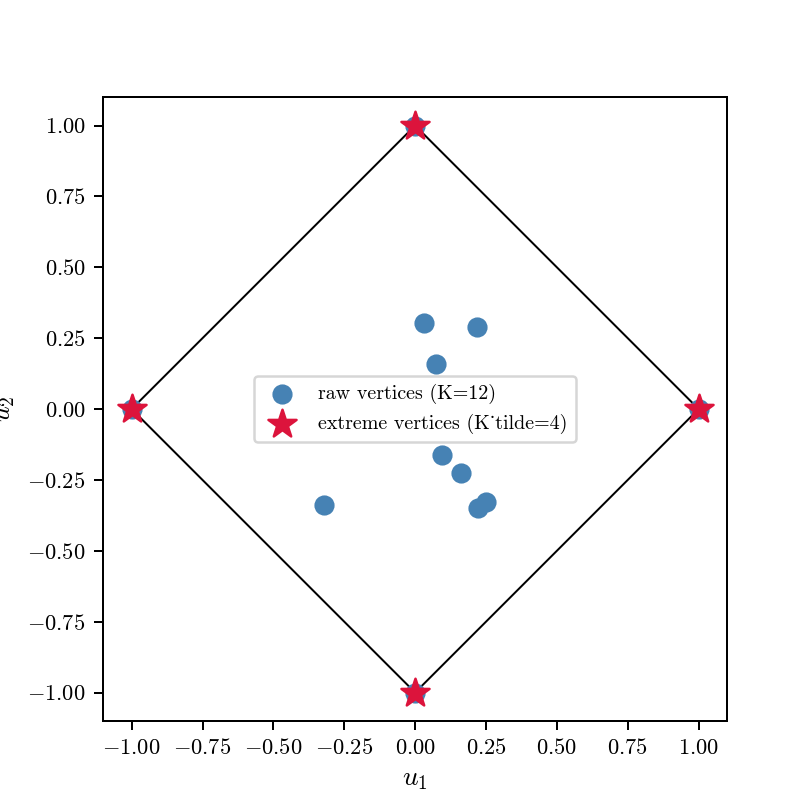
\includegraphics[width=0.65\textwidth]{figures/control_set.png}
	\caption{Raw vertex set $U_{\mathrm{raw}}$ ($K_{\mathrm{raw}}=12$, blue circles: the
		four true extreme vertices of the $\ell^1$ diamond plus eight redundant
		interior points) and the four extreme vertices $\widetilde{K}=4$ recovered
		by Quickhull (red stars), together with the convex hull of $U_{\mathrm{raw}}$.}
	\label{fig:control-set}
\end{figure}

Since $B = I_2$, the offline-reduced set is
$\widetilde{U} = \{e_1, -e_1, e_2, -e_2\}$,
and the vertex set at each collocation point is built online as
\begin{equation}
  \label{eq:Vtilde-online}
  \widetilde{V}(x_\theta(t_i))
  = \bigl\{Ax_\theta(t_i) + \tilde{u}_k\bigr\}_{k=1}^{\widetilde{K}}.
\end{equation}
The projection $\Pi_{F_i}\!\bigl(\dot{x}_\theta(t_i)\bigr)$
is then computed by solving the QP~\eqref{eq:projection-as-qp}
with $\widetilde{K} = 4$ variables using the SLSQP method.


\paragraph{Neural network and training}
The trial solution takes the form
\begin{equation}
  \label{eq:trial-linear}
  x_\theta(t) = x_0 + t\,N_\theta(t),
\end{equation}
where $N_\theta : \mathbb{R} \to \mathbb{R}^2$ is a fully connected neural
network with $\tanh$ activation, three hidden layers of width 64, and
Glorot-normal initialization.
The parametrization~\eqref{eq:trial-linear} enforces $x_\theta(0) = x_0$
exactly for every $\theta$, so the DR-PINN loss reduces to the pure inclusion
term
\begin{equation}
  \label{eq:loss-linear}
  \mathcal{L}(\theta)
  = \frac{1}{N} \sum_{i=1}^{N}
    \dist^2\!\bigl(\dot{x}_\theta(t_i),\, F(x_\theta(t_i))\bigr),
\end{equation}
evaluated at $N = 300$ collocation points distributed uniformly on $[0, T]$.
Training is performed with the Adam optimizer at learning rate $10^{-3}$ for
$1\,000$ epochs. Figure~\ref{fig:loss-linear} shows the inclusion loss $\mathcal{L}(\theta)$
of~\eqref{eq:loss-linear} along training. Starting from
$\mathcal{L}(\theta) \approx 2.1\times10^{-1}$ at initialization, the loss
decreases to $1.2\times10^{-12}$ after $1\,000$ epochs, confirming that the
learned velocity $\dot x_\theta(t)$ becomes admissible, i.e.\
$\dot x_\theta(t) \in F(x_\theta(t))$, at (numerically) every collocation
point.

\begin{figure}[htbp]
	\centering
	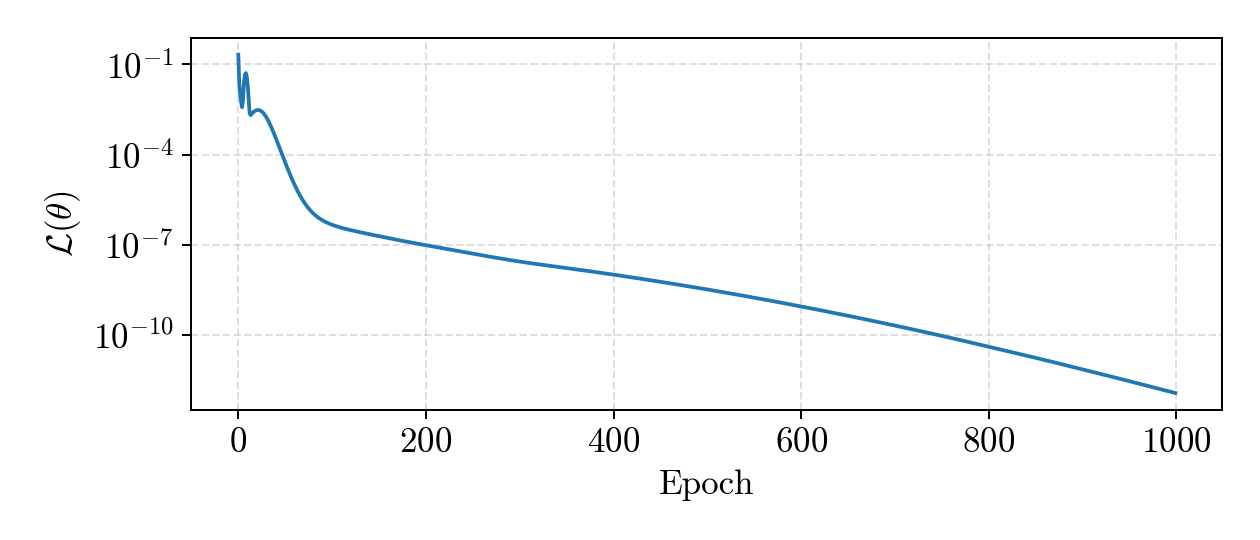
\includegraphics[width=\textwidth]{figures/loss_single.png}
	\caption{Training history of the inclusion loss $\mathcal{L}(\theta)$ for
		the single DR-PINN of this section (semi-logarithmic scale).}
	\label{fig:loss-linear}
\end{figure}

\paragraph{Reference reachable tube}
A reference inner approximation of the reachable tube
\begin{equation}
  \label{eq:reachable-tube}
  \mathcal{R}(t)
  =
  \bigl\{
    x(t)
    :
    \dot{x}(s) = Ax(s) + Bu(s),\;
    u(s) \in U \text{ a.e.},\;
    x(0) = x_0
  \bigr\}
\end{equation}
is constructed by integrating the ODE $\dot{x} = Ax + Bu$ with two families
of admissible controls:
\begin{enumerate}
	\item[(a)] \emph{Constant bang-bang controls}: one trajectory per extreme
	vertex $u_k \in \widetilde{U}$, totalling four reference trajectories.
	By Pontryagin's maximum principle, since the Hamiltonian of a linear
	system is affine in the control, its maximum over the polytope $U$ is
	attained at an extreme point; hence the boundary of $\mathcal{R}(t)$ is
	traced by bang-bang controls taking values in $\widetilde{U}$
	(see, e.g., \cite{LeeMarkus1967}, Chapter 4, or \cite{aubin_cellina_1984},
	Chapter 8). This family covers the boundary of $\mathcal{R}(t)$.
  \item[(b)] \emph{Piecewise-constant random controls}: 300 trajectories obtained
        by randomly switching among the vertices of $U$ at uniformly
        distributed times, each trajectory integrated with a fifth-order
        Runge--Kutta scheme (relative tolerance $10^{-9}$, absolute
        tolerance $10^{-11}$).
        This family densely samples the interior of $\mathcal{R}(t)$.
\end{enumerate}
The union of all 304 trajectories evaluated on a uniform time grid of 200
points constitutes the reference tube used for comparison.

Figure~\ref{fig:phase-linear} overlays the trained trajectory $x_\theta(t)$
with the reference reachable tube $\mathcal{R}(t)$ of~\eqref{eq:reachable-tube}:
the left panel shows the phase portrait, the right panel the two state
components against time. The learned trajectory remains inside the reference
tube throughout $[0,T]$, an empirical illustration of
Theorem~\ref{thm:consistency}: a vanishing inclusion loss produces an
admissible trajectory. 
\begin{figure}[htbp]
	\centering
	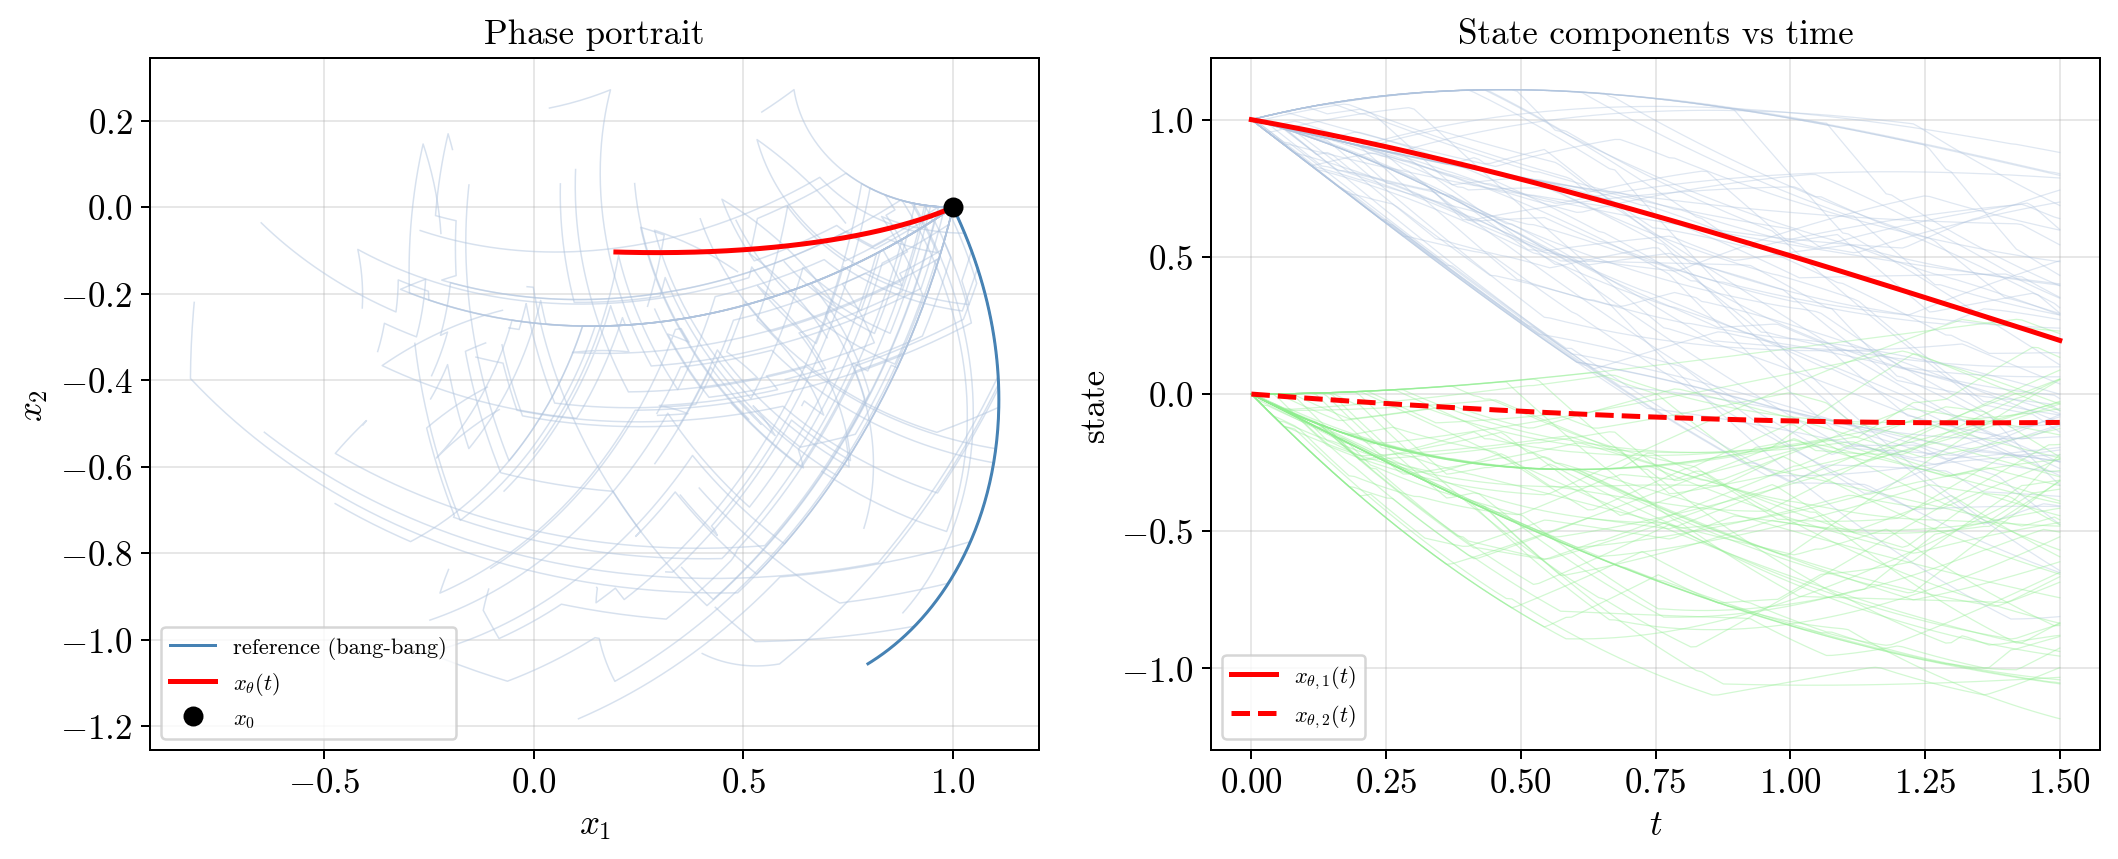
\includegraphics[width=\textwidth]{figures/trajectory_vs_tube.png}
	\caption{Phase portrait (left) and state components versus time (right)
		for the trained trajectory $x_\theta(t)$, compared with the reference
		reachable tube $\mathcal{R}(t)$ (304 trajectories, light blue) and one
		representative bang-bang extremal (dark blue).}
	\label{fig:phase-linear}
\end{figure}

\paragraph{Ensemble and Hausdorff metric}
Since a single DR-PINN approximates one element of the solution set
$\mathcal{S}(x_0)$ (cf.\ Section~\ref{subsec:consistency}), its distance to the
reference tube is not, by itself, a robust check: we train an
ensemble of $n_{\mathrm{ens}} = 5$ networks with different random seeds and
average the resulting metric over the ensemble.
The PINN reachable tube at time $t$ is defined as
\[
  \mathcal{R}_\theta(t) = \bigl\{x_\theta^{(s)}(t) : s = 1,\dots,n_{\mathrm{ens}}\bigr\}.
\]
Admissibility is measured by the one-sided Hausdorff distance
\[
  d_H^+\!\bigl(\mathcal{R}_\theta(t),\,\mathcal{R}(t)\bigr)
  = \max_{a \in \mathcal{R}_\theta(t)}\min_{b \in \mathcal{R}(t)}\|a-b\|,
\]
which quantifies how far the ensemble trajectories lie from the reference
tube, averaged over the ensemble and over the time grid.
Averaging the one-sided Hausdorff distance
$d_H^+(\mathcal{R}_\theta(t),\mathcal{R}(t))$ over the ensemble of
$n_{\mathrm{ens}}=5$ networks and over the time grid gives
\[
  \overline{d_H^+}(\mathcal{R}_\theta,\mathcal{R}) = 0.0445,
\]
which is small relative to the scale of the problem (the control set $U$ and
the reachable tube $\mathcal{R}(t)$ both have diameter of order $1$), showing
that the ensemble reliably produces admissible trajectories regardless of the
random initialization.

\paragraph{Computational scalability}
Computational efficiency is assessed by a scalability study that varies
$K_{\mathrm{raw}} \in \{8, 16, 32, 64, 128\}$ (at fixed $d = 2$) and
$d \in \{2, 4, 6, 8\}$ (at fixed $K_{\mathrm{raw}} = 32$), comparing the
per-epoch training time with and without the Quickhull reduction.
Table~\ref{tab:quickhull-K} lists the number of extreme vertices
$\widetilde{K}$ recovered by Quickhull for each raw vertex-set size
$K_{\mathrm{raw}} \in \{8,16,32,64,128\}$, at fixed $d=2$. As in the main
example, the raw point cloud consists of a fixed hexagonal boundary (six true
extreme points) plus $K_{\mathrm{raw}}-6$ redundant interior points, so
$\widetilde{K}=6$ irrespective of $K_{\mathrm{raw}}$.

\begin{table}[htbp]
  \centering
  \begin{tabular}{lccccc}
    \toprule
    $K_{\mathrm{raw}}$ & 8 & 16 & 32 & 64 & 128 \\
    \midrule
    $\widetilde{K}$    & 6 & 6  & 6  & 6  & 6   \\
    \bottomrule
  \end{tabular}
  \caption{Extreme vertices $\widetilde{K}$ recovered by Quickhull as
  $K_{\mathrm{raw}}$ grows, at fixed $d=2$.}
  \label{tab:quickhull-K}
\end{table}

For the dimension sweep, a fresh random drift matrix $A_d \in
\mathbb{R}^{d\times d}$ is generated for each $d \in \{2,4,6,8\}$, together
with a random polytope of $K_{\mathrm{raw}}=32$ vertices. To guarantee that
the uncontrolled system $\dot x = A_d x$ remains asymptotically stable
regardless of the random draw, $A_d$ is constructed by first sampling a
Gaussian matrix $G$ (i.i.d.\ entries $\mathcal{N}(0,0.3^2)$) and then
shifting its diagonal,
\[
  (A_d)_{ii} = G_{ii} - \Bigl(\textstyle\sum_{j=1}^{d}|G_{ij}| + 0.5\Bigr),
  \qquad
  (A_d)_{ij} = G_{ij} \ \ (j \neq i).
\]
By the Gershgorin circle theorem, every eigenvalue $\lambda$ of $A_d$ lies in
a disc centred at the real number $(A_d)_{ii}$ with radius
$R_i = \sum_{j\neq i}|(A_d)_{ij}| = \sum_{j\neq i}|G_{ij}|$, so
\[
  \operatorname{Re}(\lambda) \;\le\; (A_d)_{ii} + R_i
  \;=\; G_{ii} - |G_{ii}| - 0.5
  \;\le\; -0.5
\]
for every row $i$, since $G_{ii}\le |G_{ii}|$. Hence every eigenvalue of
$A_d$ has real part at most $-0.5$, for every random draw and every $d$: the
construction guarantees a uniform stability margin without ever having to
reject an unstable sample.

Table~\ref{tab:quickhull-d} shows that, unlike the $K$-sweep, $\widetilde{K}$
now grows with $d$: a random point cloud in higher dimensions has a larger
fraction of extreme points, and at $d=6,8$ all $32$ raw vertices are already
extreme, so no reduction is possible.

\begin{table}[htbp]
  \centering
  \begin{tabular}{lcccc}
    \toprule
    $d$             & 2  & 4  & 6  & 8  \\
    \midrule
    $\widetilde{K}$ & 12 & 23 & 32 & 32 \\
    \bottomrule
  \end{tabular}
  \caption{Extreme vertices $\widetilde{K}$ recovered by Quickhull as the
  state dimension $d$ grows, at fixed $K_{\mathrm{raw}}=32$.}
  \label{tab:quickhull-d}
\end{table}

Figure~\ref{fig:scalability-linear} reports the resulting per-epoch training
time with and without the offline Quickhull reduction. As a function of
$K_{\mathrm{raw}}$ (left panel), the Quickhull-reduced training time stays
essentially flat, between $760$ and $850\,$ms, while the unreduced QP grows
from $888\,$ms to $7.07\,$s at $K_{\mathrm{raw}}=128$ -- an $8.3\times$
slowdown -- because the QP of Section~\ref{sec:projection-extreme-points}
then has $128$ variables instead of $6$. As a function of $d$ (right panel),
the benefit shrinks as $\widetilde{K}$ approaches $K_{\mathrm{raw}}$: at
$d=6$ and $d=8$, where Table~\ref{tab:quickhull-d} shows no reduction is
achieved, the Quickhull-reduced time ($1.61\,$s, $1.48\,$s) is no longer
lower than the unreduced time ($1.56\,$s in both cases), since the
preprocessing step then adds overhead without shrinking the downstream QP.

\begin{figure}[htbp]
  \centering
  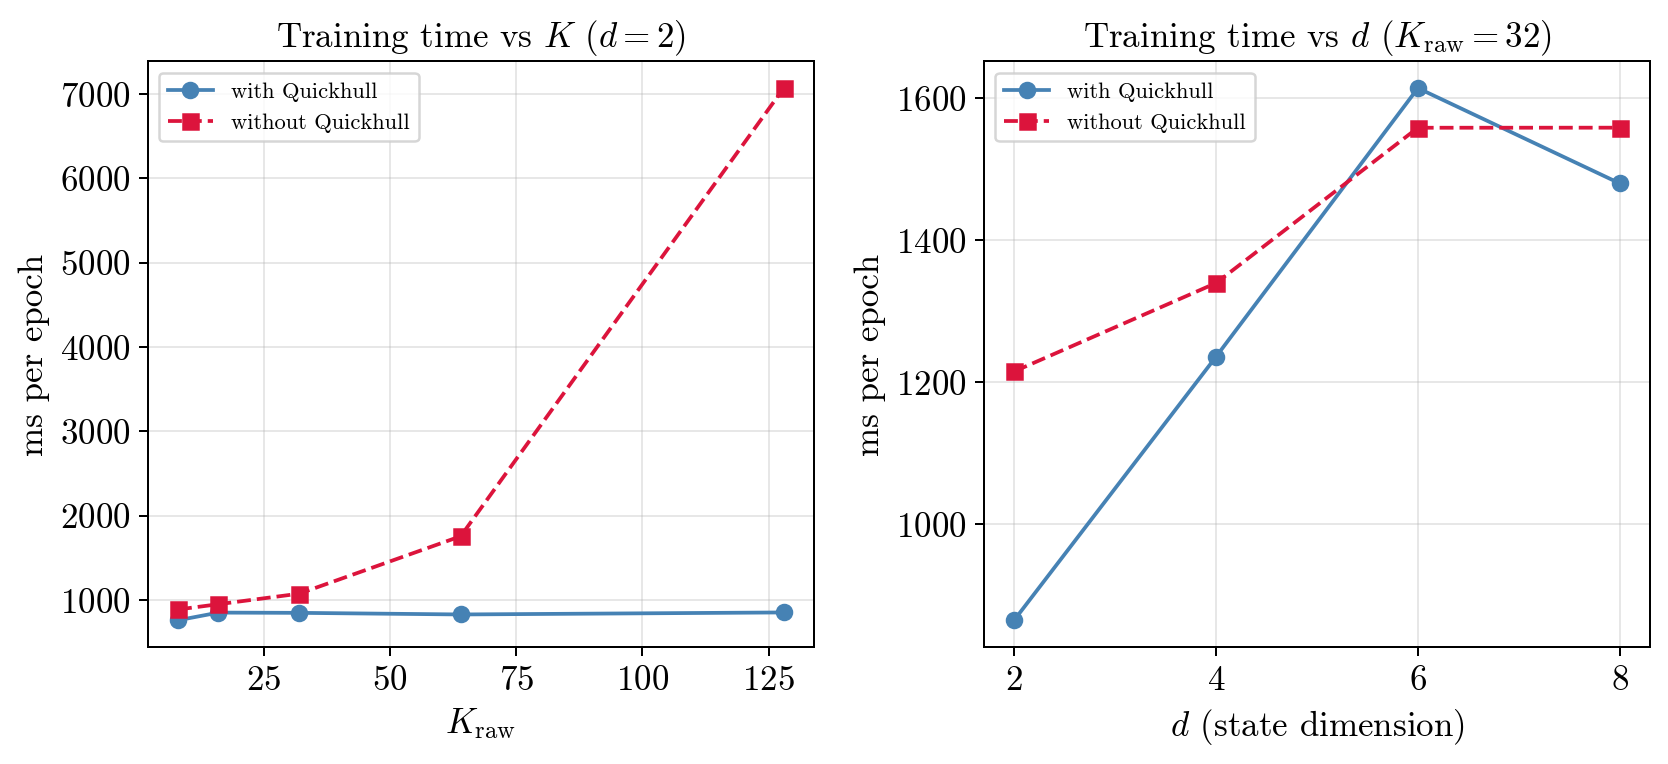
\includegraphics[width=\textwidth]{figures/scalability.png}
  \caption{Per-epoch training time with (blue) and without (red) the offline
  Quickhull reduction. Left: as a function of $K_{\mathrm{raw}}$ at fixed
  $d=2$ (Table~\ref{tab:quickhull-K}). Right: as a function of the state
  dimension $d$ at fixed $K_{\mathrm{raw}}=32$ (Table~\ref{tab:quickhull-d}).}
  \label{fig:scalability-linear}
\end{figure}

%% ------------------------------------------------------------
\subsection{A Planar Differential Inclusion with a Rotating Ellipsoidal Control Constraint}
\label{subsec:rotating-ellipsoidal}
%% ------------------------------------------------------------

\paragraph{Problem formulation}
The two examples of Sections~\ref{subsec:linear-control}
and~\ref{subsec:parabolic-PDI} enforce the inclusion by \emph{minimizing}
the distance residual. This second ODE example illustrates the
complementary strategy anticipated in
Section~\ref{sec:description-formulation}: when the admissible set has a
tractable parametric description, admissibility can be built into the
parametrization itself, so that the distance residual vanishes
\emph{identically} along every candidate trajectory and the remaining
degrees of freedom can be used to select a specific element of the
solution set $\mathcal{S}(x_0)$ --- here, the trajectory steering the
state closest to a prescribed terminal point. This makes concrete the
non-uniqueness discussion of Section~\ref{subsec:consistency}: the
distance-residual loss guarantees convergence to \emph{some} admissible
trajectory, whereas a hard-admissible parametrization allows one to
optimize \emph{which} one.

We consider trajectories $x:[0,T]\to\mathbb{R}^2$ of the differential
inclusion
\begin{equation}
	\label{eq:ellipse-inclusion}
	\dot{x}(t)\in F(t,x(t)) = g(t,x(t))+E(t),
	\qquad x(0)=x_0,
\end{equation}
whose admissible-velocity set is of Minkowski type: a nonlinear,
nonautonomous drift
\begin{equation}
	\label{eq:ellipse-drift}
	g(t,x)=
	\begin{pmatrix}
		\sin(x_1)+0.15\cos\bigl(\tfrac{2\pi t}{T}\bigr)\\[2mm]
		0.5\cos(x_2)-0.20\sin\bigl(\tfrac{2\pi t}{T}\bigr)
	\end{pmatrix},
	\qquad x=(x_1,x_2)^{\top},
\end{equation}
translated by a compact, convex, \emph{time-dependent} control set
$E(t)$, a rotating ellipse defined below. Equivalently, admissible
trajectories are exactly the solutions of the controlled system
\begin{equation}
	\label{eq:ellipse-controlled}
	\dot{x}(t)=g(t,x(t))+\xi(t),
	\qquad \xi(t)\in E(t)\ \text{ a.e.\ on } [0,T],
\end{equation}
where $\xi$ is a measurable selector of $t\mapsto E(t)$. Since
$E(t)$ does not depend on the state, this example falls into
regime~(a) of Section~\ref{sec:projection-extreme-points}; however,
unlike the polytopic set of Section~\ref{subsec:linear-control}, the
projection onto an ellipse admits no closed form (it requires the
solution of a scalar secular equation), which makes the hard-admissible
route particularly attractive here. We take $T=3$ and $x_0=(0,0)^{\top}$.

\paragraph{The rotating ellipsoidal control set}
For $t\in[0,T]$, let
\begin{equation}
	\label{eq:ellipse-axes}
	a(t)=0.3+0.4\Bigl|\sin\Bigl(\frac{\pi t}{T}\Bigr)\Bigr|,
	\qquad
	b(t)=0.15+0.25\Bigl|\cos\Bigl(\frac{\pi t}{T}\Bigr)\Bigr|,
	\qquad
	\varphi(t)=\frac{\pi t}{T},
\end{equation}
and let $R_{\varphi(t)}$ denote the rotation by the angle $\varphi(t)$.
The control set is the (filled) rotating ellipse
\begin{equation}
	\label{eq:ellipse-set}
	E(t)=\Bigl\{R_{\varphi(t)}
	\begin{pmatrix}u\\w\end{pmatrix}\in\mathbb{R}^2:
	\frac{u^2}{a(t)^2}+\frac{w^2}{b(t)^2}\leq 1\Bigr\},
\end{equation}
which is nonempty, compact, and convex for every $t$, with semi-axes and
orientation varying continuously in time; since $\varphi(0)=0$ and
$\varphi(T)=\pi$, the ellipse performs a half-turn over the horizon, and
the translated family $g(t,x(t))+E(t)$ traces a twisted tube of
admissible velocities along the drift curve
(Figure~\ref{fig:ellipse-tube}). Writing
$(u,w)^{\top}=R_{-\varphi(t)}\,\xi$ for the coordinates of
$\xi\in\mathbb{R}^2$ in the local frame of the ellipse, the
\emph{level function}
\begin{equation}
	\label{eq:ellipse-level}
	\ell(t,\xi)
	=\Bigl(\frac{u}{a(t)}\Bigr)^2+\Bigl(\frac{w}{b(t)}\Bigr)^2
\end{equation}
characterizes admissibility: $\xi\in E(t)$ if and only if
$\ell(t,\xi)\le1$, with $\ell=1$ on the boundary $\partial E(t)$.

\paragraph{Hard-admissible selector parametrization}
The selector is generated from $n_{\rm c}=24$ control nodes
$(p^j,\rho^j)\in\mathbb{R}^2\times\mathbb{R}$, $j=0,\dots,n_{\rm c}-1$,
linearly interpolated to the uniform time grid
$t_i=i\,\Delta t$, $i=0,\dots,n_t-1$, $\Delta t=T/(n_t-1)$, with
$n_t=120$; the low-dimensional nodal representation suppresses
artificial oscillations of the selector. From the interpolated values
$p(t_i)\in\mathbb{R}^2$, $\rho(t_i)\in\mathbb{R}$, define the unit-ball
direction and the sigmoidal radius
\begin{equation}
	\label{eq:ellipse-dir-radius}
	d(t_i)=\frac{p(t_i)}{\sqrt{\,|p(t_i)|^2+\varepsilon\,}},
	\qquad
	s(t_i)=\frac{1}{1+e^{-\rho(t_i)}}\in(0,1),
\end{equation}
with $\varepsilon=10^{-10}$ a normalization safeguard, and set
\begin{equation}
	\label{eq:ellipse-selector}
	\xi(t_i)
	=R_{\varphi(t_i)}
	\begin{pmatrix}
		s(t_i)\,a(t_i)\,d_1(t_i)\\
		s(t_i)\,b(t_i)\,d_2(t_i)
	\end{pmatrix}.
\end{equation}
Substituting \eqref{eq:ellipse-selector} into
\eqref{eq:ellipse-level} gives, for every grid point,
\begin{equation}
	\label{eq:ellipse-admissibility}
	\ell\bigl(t_i,\xi(t_i)\bigr)
	=s(t_i)^2\,|d(t_i)|^2
	\le s(t_i)^2<1,
\end{equation}
so the selector lies in the interior of $E(t_i)$ \emph{by construction},
for every value of the nodal variables: no penalty for constraint
violation is required, and the inclusion residual
$\dist\bigl(\dot x(t_i)-g(t_i,x(t_i)),E(t_i)\bigr)$ of
Section~\ref{sec:description-formulation} vanishes identically. This is
the analogue, for the inclusion constraint itself, of the hard-constraint
ansatz used for the initial condition in
Section~\ref{subsec:linear-control} and for the initial/boundary
conditions in Section~\ref{subsec:parabolic-PDI}.

\paragraph{Steering problem and discretization}
For a fixed selector, the state is propagated through
\eqref{eq:ellipse-controlled} by the classical fourth-order
Runge--Kutta scheme on the grid $\{t_i\}$, with $\xi$ evaluated between
grid points by linear interpolation. The nodal variables
$z=(p^0,\dots,p^{n_{\rm c}-1},\rho^0,\dots,\rho^{n_{\rm c}-1})
\in\mathbb{R}^{3n_{\rm c}}=\mathbb{R}^{72}$
are chosen by minimizing
\begin{equation}
	\label{eq:ellipse-cost}
	J(z)=\lambda_{\rm f}\,\bigl|x_z(T)-x_{\rm f}\bigr|^2
	+\lambda_{\xi}J_{\xi}(z)+\lambda_{\rm s}J_{\rm s}(z)
	+\lambda_{\rm c}J_{\rm c}(z)+\lambda_{\rm b}J_{\rm b}(z)
	+\lambda_{\rm u}J_{\rm u}(z),
\end{equation}
where $x_z$ denotes the discrete trajectory induced by $z$, the terminal
term steers the state to a prescribed target $x_{\rm f}$, and the
regularizers are the mean level
$J_{\xi}=\frac{1}{n_t}\sum_i\ell(t_i,\xi_z(t_i))$
(discouraging boundary-hugging selectors), the mean squared first and
second discrete differences of $\xi_z$
($J_{\rm s}$, $J_{\rm c}$: smoothness and curvature), the cubic soft
barrier $J_{\rm b}=\frac{1}{n_t}\sum_i\ell(t_i,\xi_z(t_i))^3$
(penalizing boundary saturation), and the mean squared differences of
the nodal variables ($J_{\rm u}$). The weights are
$\lambda_{\rm f}=2500$, $\lambda_{\rm s}=1$, $\lambda_{\rm c}=0.2$,
$\lambda_{\rm b}=10^{-2}$, $\lambda_{\rm u}=5\cdot10^{-2}$, and the
selector-regularization weight is driven along the continuation sequence
$\lambda_{\xi}\in\{10^{-3},10^{-2},10^{-1}\}$, each stage warm-started
from the previous one and solved by L-BFGS-B.

The target must of course be chosen inside the reachable set of
\eqref{eq:ellipse-inclusion}: the drift component
$g_2=0.5\cos(x_2)-0.2\sin(2\pi t/T)$ pushes the state upward with
magnitude $\approx0.5$ near $x_2=0$, while the vertical reach of $E(t)$
oscillates between $0.15$ and $0.7$, so targets with markedly negative
$x_2$ are unreachable over $[0,T]$ (an extremal selector taking, at
every instant, the support point of $E(t)$ in the direction $-e_2$ only
attains $x_2(T)\approx-0.05$). We take
$x_{\rm f}=(1.8,\,0.1)^{\top}$, which lies inside but close to the
boundary of the reachable set: steering to it forces the selector to
operate near $\partial E(t)$ over most of the horizon, so the built-in
admissibility guarantee \eqref{eq:ellipse-admissibility} is genuinely
stressed.

\paragraph{Numerical results}
Table~\ref{tab:ellipse-continuation} reports, for each continuation
stage, the terminal mismatch and the mean and maximum of the level
function along the optimized selector. The terminal state matches the
target to $\sim10^{-5}$ at every stage, while increasing
$\lambda_{\xi}$ pulls the selector measurably towards the interior of
the ellipse (mean level decreasing from $0.940$ to $0.914$) at
essentially no cost in terminal accuracy --- the expected trade-off for
a target close to the reachable-set boundary, where near-extremal
velocities are necessary for most of the horizon.

\begin{table}[htbp]
	\centering
	\begin{tabular}{cccc}
		\toprule
		$\lambda_{\xi}$ & $|x_z(T)-x_{\rm f}|$ & mean $\ell$ & max $\ell$ \\
		\midrule
		$10^{-3}$ & $9.0\times10^{-6}$ & $0.940$ & $0.948$ \\
		$10^{-2}$ & $6.9\times10^{-6}$ & $0.919$ & $0.923$ \\
		$10^{-1}$ & $3.2\times10^{-5}$ & $0.914$ & $0.921$ \\
		\bottomrule
	\end{tabular}
	\caption{Continuation over the selector-regularization weight
		$\lambda_{\xi}$ (warm-started L-BFGS-B): terminal mismatch and level
		statistics of the optimized selector. Admissibility
		$\ell(t_i,\xi_z(t_i))<1$ holds at every grid point and every stage, by
		construction.}
	\label{tab:ellipse-continuation}
\end{table}

Figure~\ref{fig:ellipse-tube} displays the resulting geometry in the
space $(v_1,v_2,t)$ of velocities and time: the translated ellipses
$g(t_i,x_z(t_i))+E(t_i)$ form a twisted tube whose centerline is the
drift curve, and the selected velocity
$\dot{x}_z(t_i)=g(t_i,x_z(t_i))+\xi_z(t_i)$ runs inside the tube, close
to its wall, as quantified by the level statistics of
Table~\ref{tab:ellipse-continuation}. Figure~\ref{fig:ellipse-selector}
shows the same information in selector coordinates: the trajectory
$t\mapsto\xi_z(t)$ threads the rotating ellipse $E(t)$ centered at the
origin, with the color scale reporting the level
$\ell(t_i,\xi_z(t_i))$. Finally, Figure~\ref{fig:ellipse-state} shows
the optimized state trajectory from $x_0$ to $x_{\rm f}$ (left) together
with the admissibility level along the horizon (right), which stays
strictly below the boundary value $\ell=1$ at all times.

\begin{figure}[htbp]
	\centering
	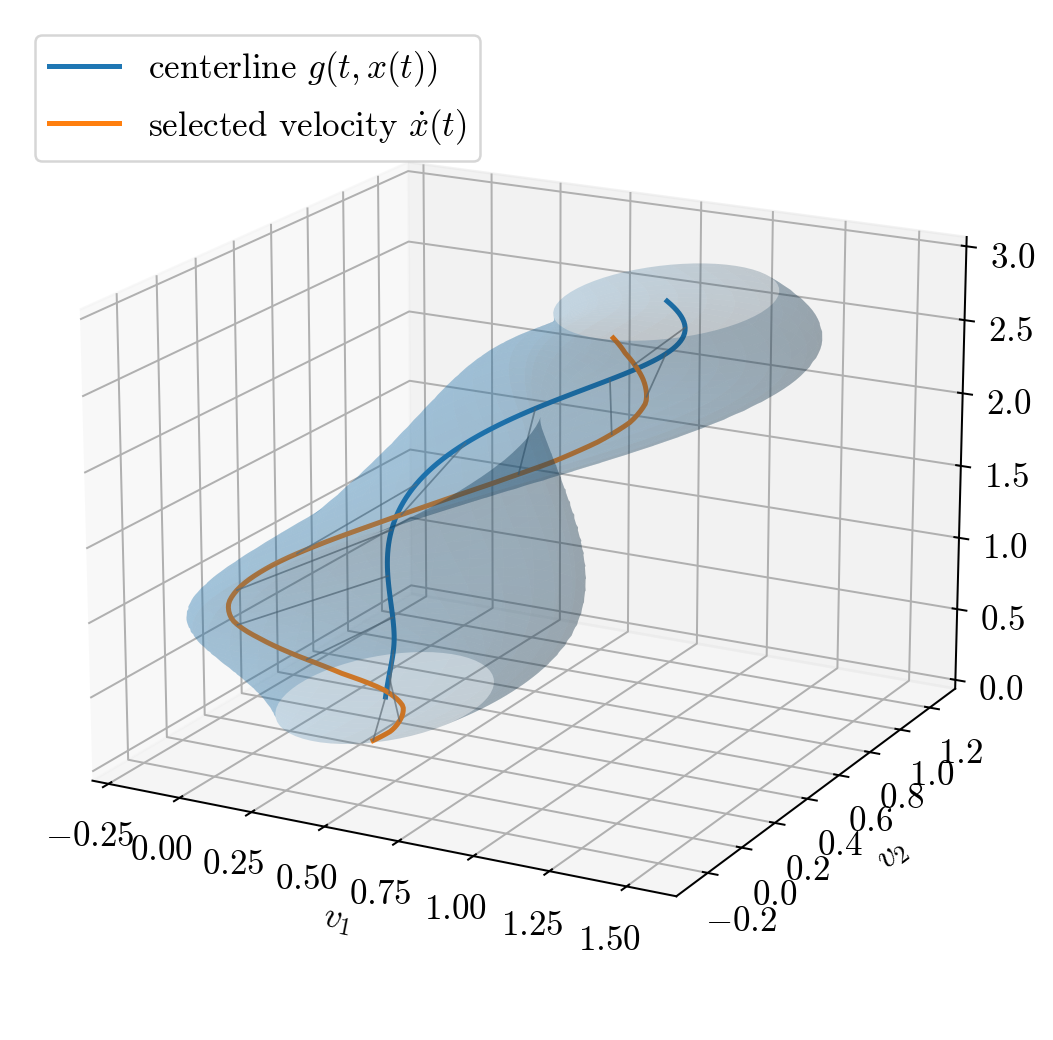
\includegraphics[width=0.78\textwidth]{figures/ellipse_velocity_tube.png}
	\caption{Admissible velocity tube of the inclusion
		\eqref{eq:ellipse-inclusion} in $(v_1,v_2,t)$ space. The surface is the
		boundary of the translated rotating ellipses $g(t,x_z(t))+E(t)$; the
		blue curve is the centerline $g(t,x_z(t))$, the orange curve the
		selected velocity $\dot{x}_z(t)$, and the grey segments the selector
		displacements $\xi_z(t_i)$.}
	\label{fig:ellipse-tube}
\end{figure}

\begin{figure}[htbp]
	\centering
	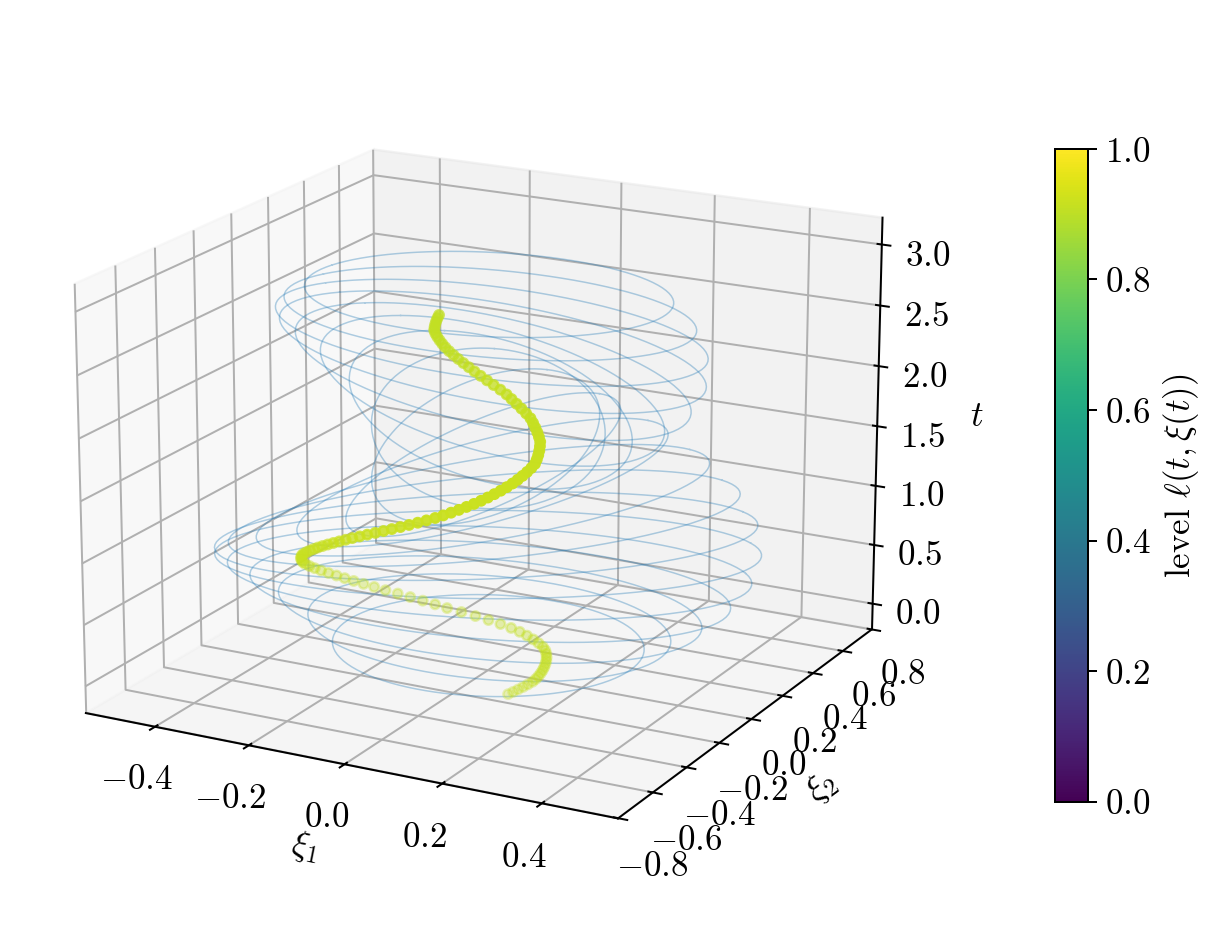
\includegraphics[width=0.78\textwidth]{figures/ellipse_selector_level.png}
	\caption{Optimized selector $\xi_z(t)$ inside the rotating control
		ellipse $E(t)$ (thin blue rings, drawn every sixth grid point). The
		color of the points encodes the level $\ell(t_i,\xi_z(t_i))$, which
		remains strictly below $1$ by construction.}
	\label{fig:ellipse-selector}
\end{figure}

\begin{figure}[htbp]
	\centering
	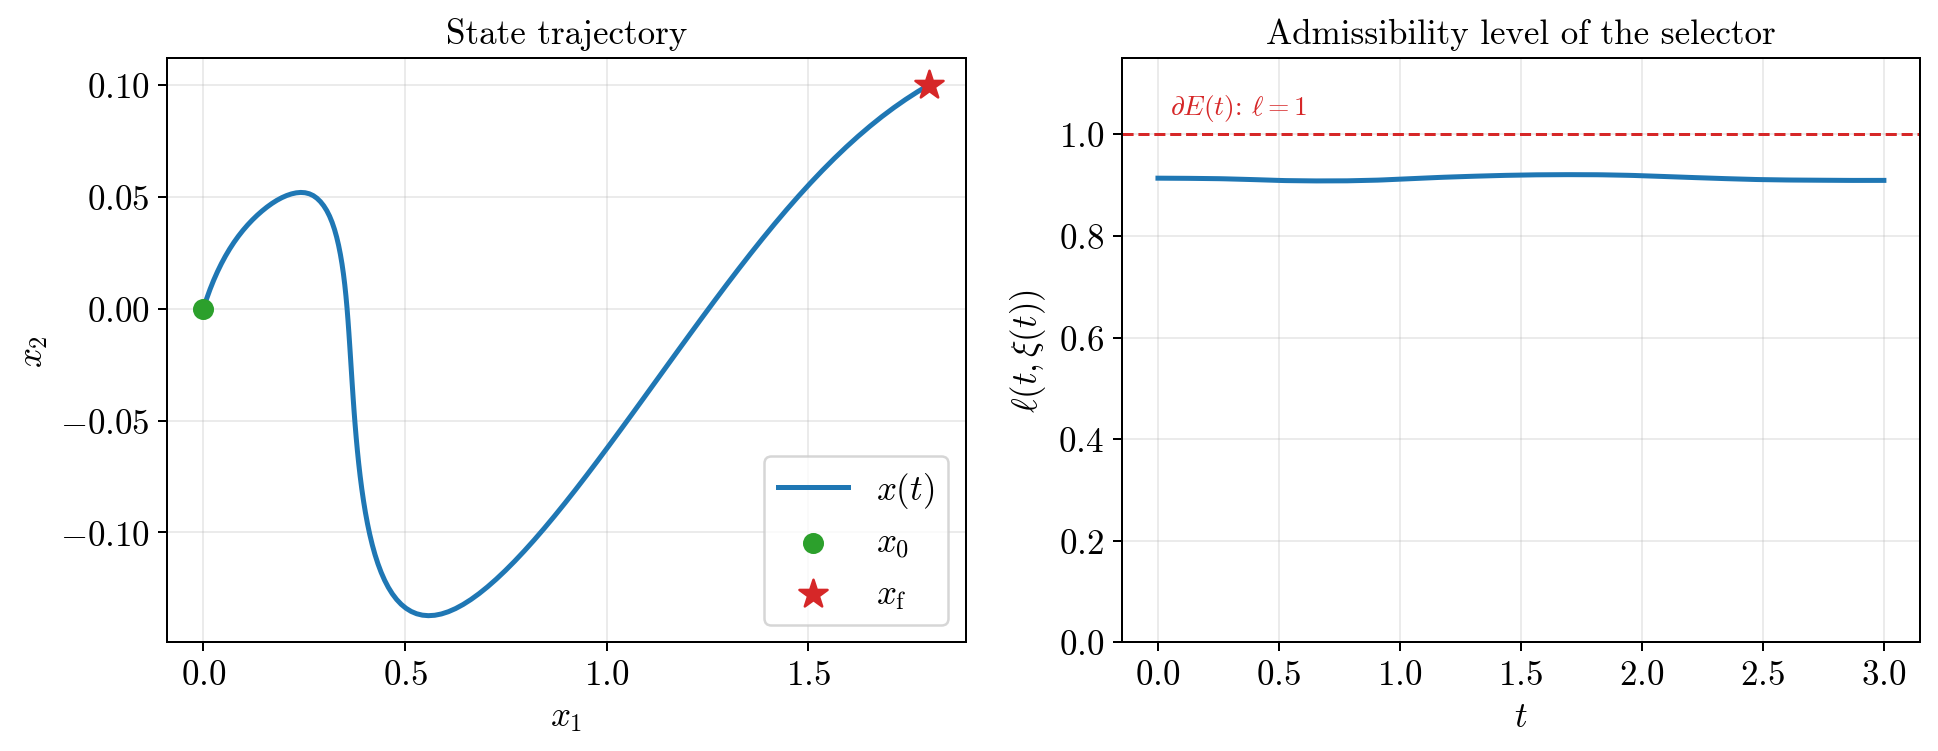
\includegraphics[width=\textwidth]{figures/ellipse_state_trajectory.png}
	\caption{Left: optimized state trajectory of
		\eqref{eq:ellipse-controlled} from $x_0=(0,0)^{\top}$ to the target
		$x_{\rm f}=(1.8,0.1)^{\top}$ (final continuation stage
		$\lambda_{\xi}=10^{-1}$, terminal mismatch $3.2\times10^{-5}$). Right: admissibility level
		$\ell(t,\xi_z(t))$ along the horizon; the dashed line marks the
		boundary value $\ell=1$ of $\partial E(t)$.}
	\label{fig:ellipse-state}
\end{figure}
\paragraph{DR-PINN companion run}
The hard-admissible selector optimization above is a direct constrained
optimal-control discretization, not a DR-PINN: it propagates the state by RK4
and makes the inclusion hold by construction. To test the distance-residual
method itself on the same benchmark, we therefore performed a separate
DR-PINN run. Because the experiment is a steering problem with prescribed
initial and terminal states, we used the endpoint-hard neural ansatz
\begin{equation}
\label{eq:ellipse-endpoint-hard}
 x_\theta(t)
 =x_0+\frac{t}{T}(x_{\rm f}-x_0)+t(T-t)N_\theta(t),
\end{equation}
where $N_\theta$ is a $3\times64$ tanh network. Hence
$x_\theta(0)=x_0$ and $x_\theta(T)=x_{\rm f}$ exactly, and the training
objective is the pure distance residual
\begin{equation}
\label{eq:ellipse-drpinn-loss}
 \mathcal{L}(\theta)
 =\frac{1}{N}\sum_{i=1}^{N}
 \dist^2\!\bigl(\dot{x}_\theta(t_i)-g(t_i,x_\theta(t_i)),E(t_i)\bigr),
\end{equation}
with $N=512$ uniform collocation points.

The projection onto an ellipse is evaluated pointwise by Newton iteration on
the secular equation
$\sum_k(\sigma_k v_k^{\rm loc}/(\sigma_k^2+\mu))^2=1$ in the local frame of
$E(t)$, with $\sigma_1=a(t)$ and $\sigma_2=b(t)$. In the backward pass the
\emph{entire projected point} $\Pi_{E(t)}(v)$ is held constant, so automatic
differentiation returns the exact envelope gradient
$2(v-\Pi_{E(t)}(v))$. Holding only the multiplier $\mu$ constant would not
give this gradient; this distinction is important in an implementation with
a numerically computed projection. A finite-difference gradient check in the
replication code gives a relative error of $7.5\times10^{-11}$.

After $7000$ Adam epochs (hold-then-decay learning rate, double precision),
the collocation loss is $1.9\times10^{-14}$. On an independent dense grid of
$2000$ time points, the mean and maximum inclusion distances are respectively
$7.1\times10^{-9}$ and $2.2\times10^{-6}$, while both endpoint errors are zero
up to machine precision. The corresponding selector has mean level $0.931$
and maximum level $1.000011$; the latter tiny overshoot is consistent with the
reported $2.2\times10^{-6}$ distance and numerical projection tolerance. Thus
the corrected distance-residual implementation does solve this benchmark as
a genuine DR-PINN. The hard-admissible selector experiment remains useful as
a complementary construction that guarantees feasibility independently of
training, but it should not itself be labelled a DR-PINN experiment.

%% ------------------------------------------------------------
\subsection{A Reaction-Diffusion Inclusion with Relay (Sliding-Mode) Feedback}
\label{subsec:parabolic-PDI}
%% ------------------------------------------------------------

As a benchmark for the parabolic setting of Section~\ref{sec:pde},
we consider the reaction-diffusion inclusion
\begin{equation}
	\label{eq:relay-pde}
	\partial_t u(t,x) - \Delta u(t,x) \in \Phi(u(t,x)),
	\qquad (t,x)\in Q = (0,T)\times\Omega,
\end{equation}
with homogeneous Dirichlet boundary condition, where
the set-valued reaction term is the relay (signum) multifunction
\begin{equation}
	\label{eq:relay-Phi}
	\Phi(s) := -\lambda\,\Sign(s)
	=
	\begin{cases}
		\{-\lambda\}, & s>0,\\[2pt]
		[-\lambda,\lambda], & s=0,\\[2pt]
		\{\lambda\}, & s<0,
	\end{cases}
	\qquad \lambda>0.
\end{equation}
Physically, \eqref{eq:relay-pde}--\eqref{eq:relay-Phi} is the parabolic
analogue of the bang-bang differential inclusion of
Section~\ref{subsec:linear-control}. Indeed, at every point $(t,x)$, instead of a
smooth reaction term, the state is driven towards the equilibrium $u\equiv0$
by a switching (relay) feedback of constant magnitude $\lambda$, exactly as
a sliding-mode controller drives a state to a manifold at constant rate
regardless of its distance to that manifold. Equivalently, $\Phi=-\lambda\,\partial|\cdot|$, so that \eqref{eq:relay-pde}
may be read as the abstract evolution inclusion
\begin{equation}
	\label{eq:relay-gradient-flow}
	\partial_t u \in -\partial E(u),
	\qquad
	E(u) = \frac12\|\nabla u\|_{L^2(\Omega)}^2 + \lambda\|u\|_{L^1(\Omega)},
\end{equation}
associated with the Dirichlet energy regularized by an $L^1$ (total-mass)
penalty, which connects this example to sparsity-promoting flows in
variational image processing and signal denoising.

We take $\Omega=(0,1)^2$ and
\begin{equation}
	\label{eq:relay-u0}
	u_0(x,y) = 16\,x(1-x)\,y(1-y),
\end{equation}
which is smooth, nonnegative, and satisfies $u_0\in H_0^1(\Omega)$, and take
$\lambda=0.6$ as a baseline value, together with a primary comparison sweep
$\lambda\in\{0.4,0.6,0.8\}$ to illustrate how the extinction time (see below)
decreases as $\lambda$ increases. The time horizon is fixed at $T=0.3$, which
is large enough that all three relay cases have visibly reached extinction while
the $\lambda=0$ (classical heat equation) case has not, making the qualitative
contrast visible in a single plot (see Figure~\ref{fig:relay-extinction-ref} below).

We check that $\Phi$ in \eqref{eq:relay-Phi} satisfies (P1)--(P3) of
Section~\ref{sec:pde-consistency}, so that Theorem~\ref{thm:consistency-parabolic}
applies to this example.
\begin{itemize}
	\item[(P1)] For every $s\in\mathbb{R}$, $\Phi(s)$ is a singleton or the
	closed interval $[-\lambda,\lambda]$, hence nonempty, closed, and convex.
	\item[(P2)] $\Phi$ is upper semicontinuous: it is locally constant on
	$\mathbb{R}\setminus\{0\}$, and at $s=0$, $\Phi(s_n)\subset[-\lambda,\lambda]=\Phi(0)$
	for every sequence $s_n\to0$. This is the standard Filippov
	regularization of the signum function \cite{Filippov1988}.
	\item[(P3)] $\sup_{r\in\Phi(s)}|r| = \lambda \le \lambda(1+|s|)$ for every
	$s\in\mathbb{R}$, so (P3) holds with $m_0=\lambda$.
\end{itemize}


\begin{remark}
	This example lies outside the scope of the existence theory of
	Theorem~\ref{thm:existence-pde}, which requires a \emph{continuous}
	selection $f(s)\in\Phi(s)$ (hypothesis~(H2$'$)). Indeed, any selection of
	$\Phi$ in \eqref{eq:relay-Phi} is forced to equal $-\lambda$ for $s>0$
	and $\lambda$ for $s<0$, hence is necessarily discontinuous at $s=0$.
	Existence of a strong solution is instead obtained from the classical
	theory of evolution equations governed by maximal monotone operators
	\cite{Brezis1973}: rewriting \eqref{eq:relay-pde} as
	$\partial_t u + \bigl(-\Delta+\lambda\,\partial|\cdot|\bigr)(u)\ni 0$,
	the operator $-\Delta+\lambda\,\partial|\cdot|$ is a sum of
	two maximal monotone (subdifferential) operators on $L^2(\Omega)$. 
\end{remark}

Next, we address the finite-time extinction issue. Multiplying \eqref{eq:relay-pde} by $u(t,\cdot)$, integrating over $\Omega$,
and using that $s\cdot v = -\lambda|s|$ for every $v\in\Phi(s)$ and every
$s\in\mathbb{R}$, a formal computation (rigorous for strong solutions) gives
the energy identity
\begin{equation}
	\label{eq:relay-energy}
	\frac12\frac{d}{dt}\|u(t)\|_{L^2(\Omega)}^2
	+
	\|\nabla u(t)\|_{L^2(\Omega)}^2
	=
	-\lambda\,\|u(t)\|_{L^1(\Omega)}.
\end{equation}
The extra dissipation term $-\lambda\|u(t)\|_{L^1(\Omega)}$, absent in the
classical heat equation ($\lambda=0$), is responsible for a qualitatively
different phenomenon: solutions of gradient flows of linear-growth
functionals such as \eqref{eq:relay-gradient-flow} are known to reach their
equilibrium in \emph{finite time} rather than merely decaying exponentially,
see \cite{AndreuCaselleMazon2004}. Once $u(t,\cdot)$ vanishes on part of
$\Omega$, the relay may ``slide'' there ($\Delta u(t,x)\in[-\lambda,\lambda]$
pointwise, consistently with $u\equiv0$), anchoring the solution at
equilibrium. This behavior is invisible to a classical pointwise-residual
PINN, which would require committing in advance to one branch of $\Phi$,
and is precisely the phenomenon this benchmark is designed to showcase.
Identity~\eqref{eq:relay-energy} also provides a solver-independent
numerical check: the decay of $\|u_\theta(t)\|_{L^2(\Omega)}^2$ along the
trained trajectory should be strictly faster than that of the corresponding
heat equation ($\lambda=0$) with the same initial datum, and the extinction
time should decrease as $\lambda$ increases.

\paragraph{Adaptive collocation sampling}
Because $\Phi$ has a genuine jump discontinuity at $s=0$, the distance
residual is hardest to drive to zero in a neighborhood of the (a priori
unknown, time-dependent) extinction front $$\{(t,x):u_\theta(t,x)=0\}.$$ This
is precisely where a smooth network output must approximate a discontinuous
right-hand side, and our experiments confirm that the residual after
training is concentrated there rather than spread uniformly over $Q$.
Purely uniform collocation under-resolves this thin, moving region relative
to its share of the loss. We therefore complement uniform collocation with
a residual/state-based adaptive refinement scheme in the spirit of the RAR
method of Lu, Meng, Mao, and Karniadakis
\cite{LuMengMaoKarniadakis2021DeepXDE}. Precisely, at fixed intervals during training,
a large pool of candidate points is drawn uniformly over $Q$, the points
with the smallest $|u_\theta|$ are retained as an auxiliary ``hard pool''
tracking the current estimate of the extinction front, and a fraction of
every subsequent training batch is drawn from this pool — refreshed
periodically as the front moves — while the remaining points continue to be
sampled uniformly over $Q$ to preserve global coverage of the domain.
In our experiments the batch size is $N_{\rm col}=2000$ collocation points per
epoch; the adaptive fraction is $30\%$ (600 points), drawn from a hard pool
of $n_{\rm pool}=4000$ candidate points selected from a uniform draw of
$20\,000$ points over $Q$ by retaining those with smallest $|u_\theta|$.
The hard pool is refreshed every $500$ training epochs as the extinction
front advances; the remaining $70\%$ of each batch is drawn uniformly over
$Q$ to preserve global domain coverage.

\paragraph{Reference solution}
Unlike the bang-bang example of Section~\ref{subsec:linear-control}, where
$F$ is genuinely multivalued and the ensemble/Hausdorff comparison of
Section~\ref{subsec:linear-control} is required, uniqueness of strong
solutions holds here: since $-\Delta+\lambda\,\partial|\cdot|$ is a sum of
maximal monotone operators, standard monotonicity arguments show that
$\tfrac{d}{dt}\|u_1-u_2\|_{L^2(\Omega)}^2\le0$ for any two strong solutions
with the same initial datum, so $\mathcal{S}(u_0)$ is a singleton. A single trained
DR-PINN can therefore be validated directly against one reference solution,
obtained by a first-order operator-splitting scheme on a uniform
$49\times49$ interior grid with time step $\Delta t=5\times10^{-4}$.
Each time step alternates an implicit diffusion solve,
$v=(I-\Delta t\,\Delta_h)^{-1}u^n$ (with the 5-point finite-difference
Laplacian $\Delta_h$ and homogeneous Dirichlet boundary conditions), and an
exact proximal step,
\[
u^{n+1}=\mathrm{sign}(v)\max(|v|-\lambda\Delta t,\,0),
\]
the pointwise proximal operator of $s\mapsto\lambda\Delta t\,|s|$.
This scheme captures finite-time extinction exactly: any grid point
for which $|v_i|\le\lambda\Delta t$ is sent to identically zero by the
soft-thresholding step.

\paragraph{Network architecture and loss function}
The trial solution takes the hard-constrained form
\begin{equation}
	\label{eq:trial-parabolic}
	u_\theta(t,x,y)
	= u_0(x,y) + t\,x(1-x)\,y(1-y)\,N_\theta(t,x,y),
\end{equation}
where $N_\theta:\mathbb{R}^3\to\mathbb{R}$ is a fully connected neural
network. The parametrization~\eqref{eq:trial-parabolic} enforces the
initial condition $u_\theta(0,\cdot)=u_0$ and the homogeneous Dirichlet
boundary condition exactly for every $\theta$ (the polynomial factor
vanishes on $\partial\Omega$), so, as in
Section~\ref{subsec:linear-control}, the DR-PINN loss reduces to the pure
inclusion term: it is~\eqref{eq:pde-distance-loss} with
$\Phi$ as in \eqref{eq:relay-Phi} and $\lambda_0=\lambda_b=0$. Since $\Phi(s)$ is an interval of
$\mathbb{R}$, the projection $\Pi_{\Phi(u_\theta(t_i,x_i))}$ needed to
evaluate the distance residual is explicit, requiring no quadratic program.
Beyond the usual comparison against the reference solver, we recommend a
diagnostic figure specific to this set-valued setting: superimposing, on a
plot of the graph of $\Phi$ (a three-branch ``staircase''), the empirical
cloud of points $\bigl(u_\theta(t_i,x_i),\,\partial_t u_\theta(t_i,x_i)-\Delta u_\theta(t_i,x_i)\bigr)$
at the collocation points after training. A well-trained network should
concentrate this cloud on the graph of $\Phi$, visually certifying that the
network has learned to select the correct branch of the relay at each
collocation point — a diagnostic with no counterpart in classical
single-valued PINNs.



\paragraph{Numerical results}

Figure~\ref{fig:relay-extinction-ref} displays the $L^2(\Omega)$-norm decay curves
for the reference solver with $\lambda\in\{0,0.4,0.6,0.8\}$ over $[0,T]$.
The contrast is sharp: the classical heat equation ($\lambda=0$) decays
exponentially and remains well above zero at $t=T=0.3$, while all three
relay cases reach exact numerical extinction within $[0,0.19]$, with the
extinction time decreasing monotonically as $\lambda$ increases.
Table~\ref{tab:relay-extinction} records the reference extinction times and
those detected by the trained DR-PINNs.

\begin{figure}[htbp]
  \centering
  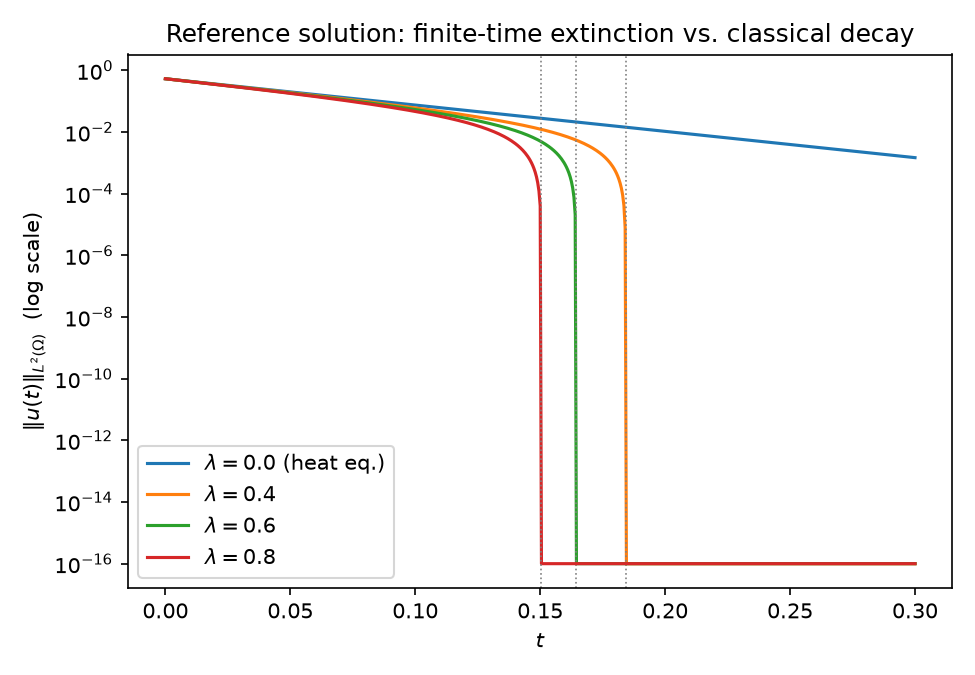
\includegraphics[width=0.72\textwidth]{figures/reference_extinction_curves.png}
  \caption{Reference solution: $\|u(t)\|_{L^2(\Omega)}$ on a log scale for
    $\lambda\in\{0,0.4,0.6,0.8\}$. The vertical dotted lines mark the finite-time
    extinction instants $t^*$ of the three relay cases; the $\lambda=0$ heat-equation
    curve does not extinguish within $[0,T]$. Curves are clipped below $10^{-6}$
    for readability; after extinction the reference norm is exactly zero
    (drop below the axis).}
  \label{fig:relay-extinction-ref}
\end{figure}

\begin{table}[htbp]
  \centering
  \begin{tabular}{cccc}
    \toprule
    $\lambda$ & $t^*_{\rm ref}$ & $t^*_{\rm DR\text{-}PINN}$ & relative error \\
    \midrule
    0.4 & 0.1845 & 0.1900 & $3.0\%$ \\
    0.6 & 0.1645 & 0.1725 & $4.9\%$ \\
    0.8 & 0.1505 & 0.1625 & $8.0\%$ \\
    \bottomrule
  \end{tabular}
  \caption{Reference and DR-PINN extinction times $t^*$ for the primary sweep
    $\lambda\in\{0.4,0.6,0.8\}$. The DR-PINN extinction time is defined as
    the first evaluation instant at which $\|u_\theta(t)\|_{L^2(\Omega)}<10^{-3}$.}
  \label{tab:relay-extinction}
\end{table}

The network for the baseline case $\lambda=0.6$ is a fully connected $\tanh$
network with five hidden layers of width $128$ and Glorot-normal initialization,
trained for $40\,000$ epochs with the Adam optimizer under a hold-then-decay
learning-rate schedule: the rate is held at $2\times10^{-3}$ for the first
$5\,000$ epochs and then decayed exponentially with rate $0.85$ per
$3\,000$ steps. The same architecture and schedule are used for each $\lambda$
in the primary sweep.

Figure~\ref{fig:relay-training} shows the training and validation loss curves
for the baseline run ($\lambda=0.6$). After a brief initial plateau at
$\mathcal{L}\approx 20$ (epochs $0$--$4\,500$), the loss drops abruptly by
roughly two orders of magnitude and then decreases steadily for the remainder
of training, reaching a final validation loss of $3.9\times10^{-1}$.
Training and validation curves track each other closely throughout,
indicating no overfitting.

\begin{figure}[htbp]
  \centering
  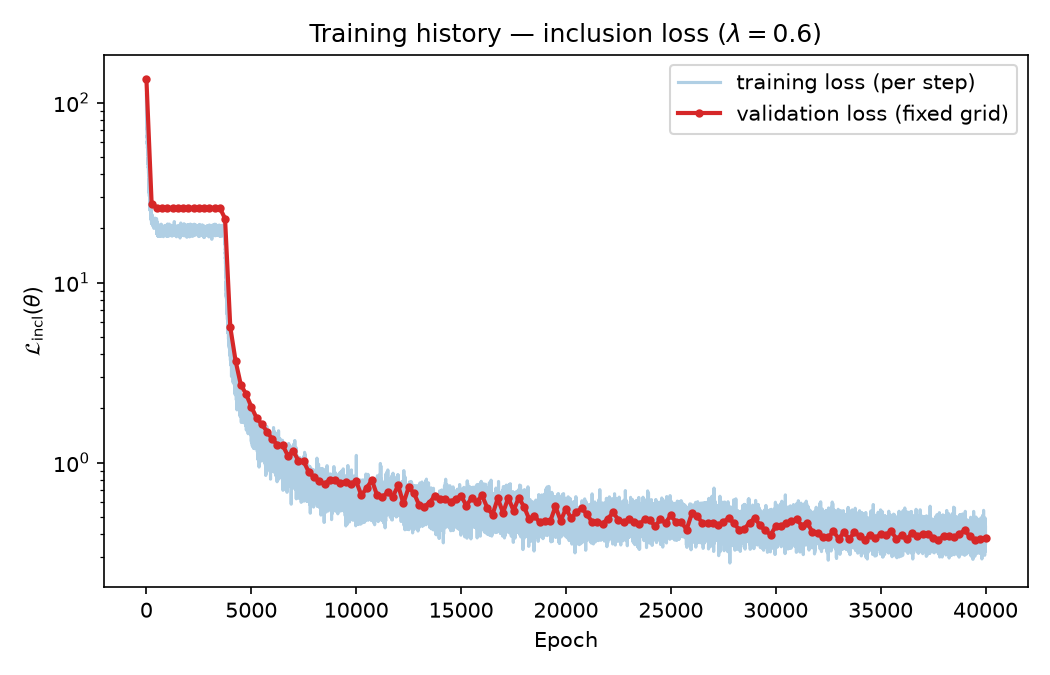
\includegraphics[width=0.80\textwidth]{figures/training_history_relay.png}
  \caption{Training history of the inclusion loss $\mathcal{L}_{\rm incl}(\theta)$
    for the baseline DR-PINN ($\lambda=0.6$, $40\,000$ epochs). The training
    loss per step (light blue) and the validation loss evaluated on a fixed
    batch of $4\,000$ points (red markers, every $250$ epochs) track each
    other closely; the abrupt drop near epoch $4\,500$ marks the escape from
    the initial plateau.}
  \label{fig:relay-training}
\end{figure}

Figure~\ref{fig:relay-vs-ref} compares the DR-PINN against the reference
solution for $\lambda=0.6$. The left panel overlays the $L^2(\Omega)$-norm
decay curves: the two coincide to within a line width for $t\lesssim0.16$,
with a maximum relative discrepancy of $0.76\%$ over $[0,T]$.
After the reference solution extinguishes at $t^*_{\rm ref}=0.1645$ (dropping
to machine zero), the DR-PINN norm stabilizes at $\approx10^{-4}$, since a
smooth network cannot represent an identically zero function after a sharp
front. The right panel shows the pointwise absolute error
$|u_\theta-u_{\rm ref}|$ at $t=T=0.3$: the error is at most
$2\times10^{-3}$, smooth, and concentrated at the domain centre, a pattern
consistent with the residual of a smooth approximation of the trivial
solution $u\equiv0$ after extinction.

\begin{figure}[htbp]
  \centering
  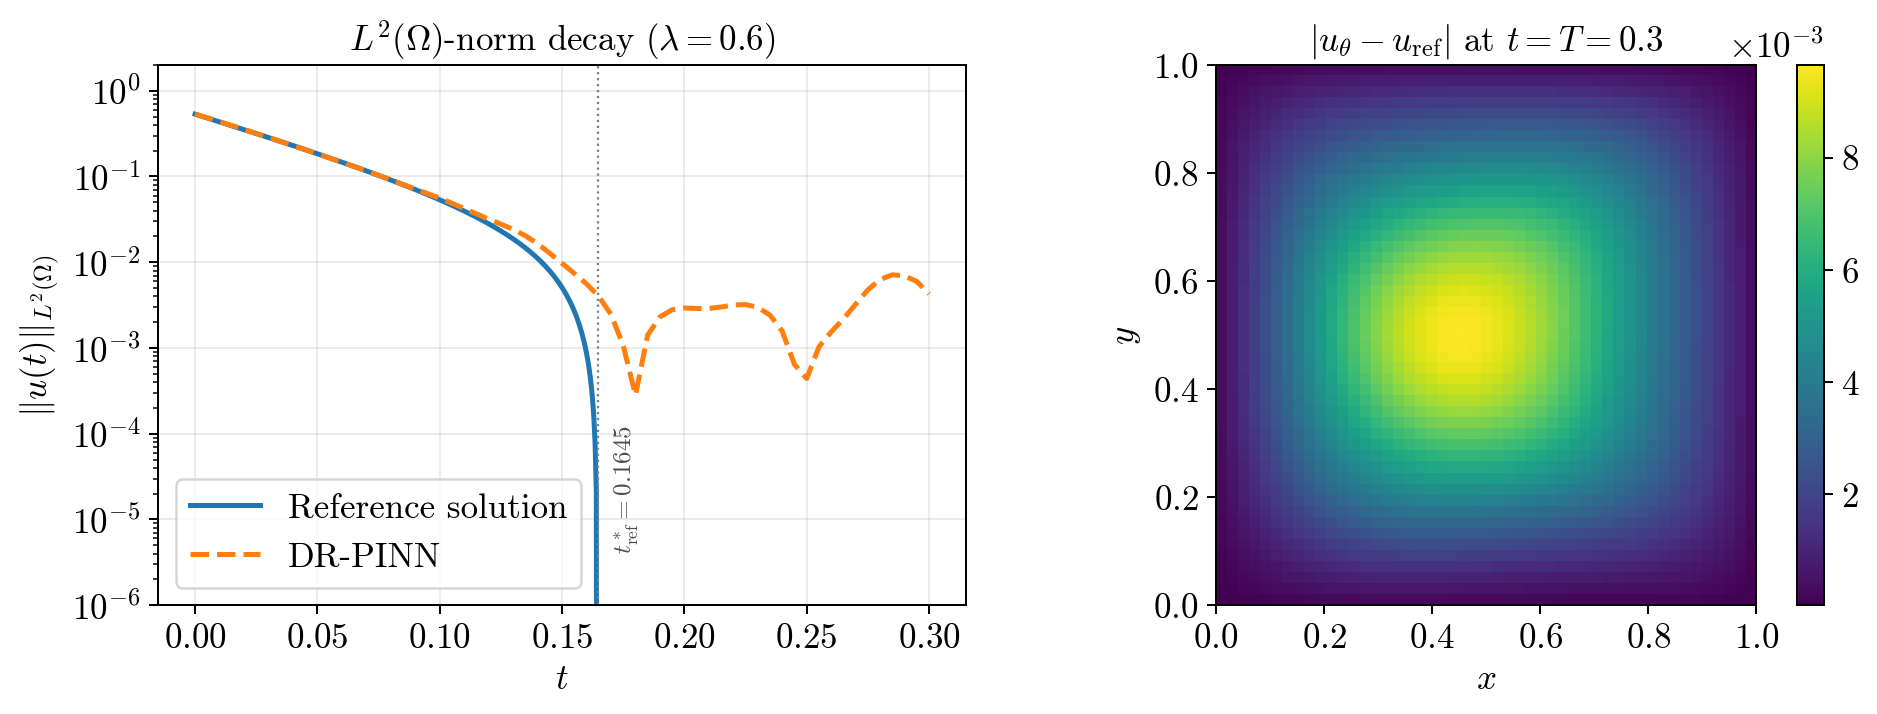
\includegraphics[width=\textwidth]{figures/dr_pinn_vs_reference.png}
  \caption{Validation of the DR-PINN against the reference solution
    ($\lambda=0.6$). Left: $L^2(\Omega)$-norm decay on a log scale (clipped
    below $10^{-6}$ for readability); the
    dotted vertical line marks the reference extinction time
    $t^*_{\rm ref}=0.1645$. Right: pointwise error $|u_\theta-u_{\rm ref}|$
    at $t=T=0.3$; the maximum error is $\approx2\times10^{-3}$.}
  \label{fig:relay-vs-ref}
\end{figure}

Figure~\ref{fig:relay-branch} shows the branch-selection diagnostic for the
baseline run. For state values $s=u_\theta(t,x,y)\gtrsim0.05$, the cloud of
operator values $z=\partial_tu_\theta-\Delta u_\theta$ concentrates tightly on
the branch $z=-\lambda=-0.6$ of the graph of $\Phi$, confirming that the
network has correctly selected the positive branch over most of $Q$.
No collocation points appear with $s<0$: since $u_0\ge0$ and the relay
feedback pushes $u$ towards zero without reversing sign, the exact solution
satisfies $u(t,\cdot)\ge0$ for all $t$, and the trained network reproduces
this property implicitly. Near $s\approx0$, corresponding to the extinction
front, the cloud disperses vertically with values of $z$ reaching up to $7$,
far above the segment $[-\lambda,\lambda]$ of the graph of $\Phi$. This
scatter is a direct consequence of the jump discontinuity of $\Phi$ at
$s=0$: no smooth network output can resolve a discontinuous right-hand side
pointwise, and the adaptive hard pool concentrates collocation points precisely
where the residual is hardest to reduce.

\begin{figure}[htbp]
  \centering
  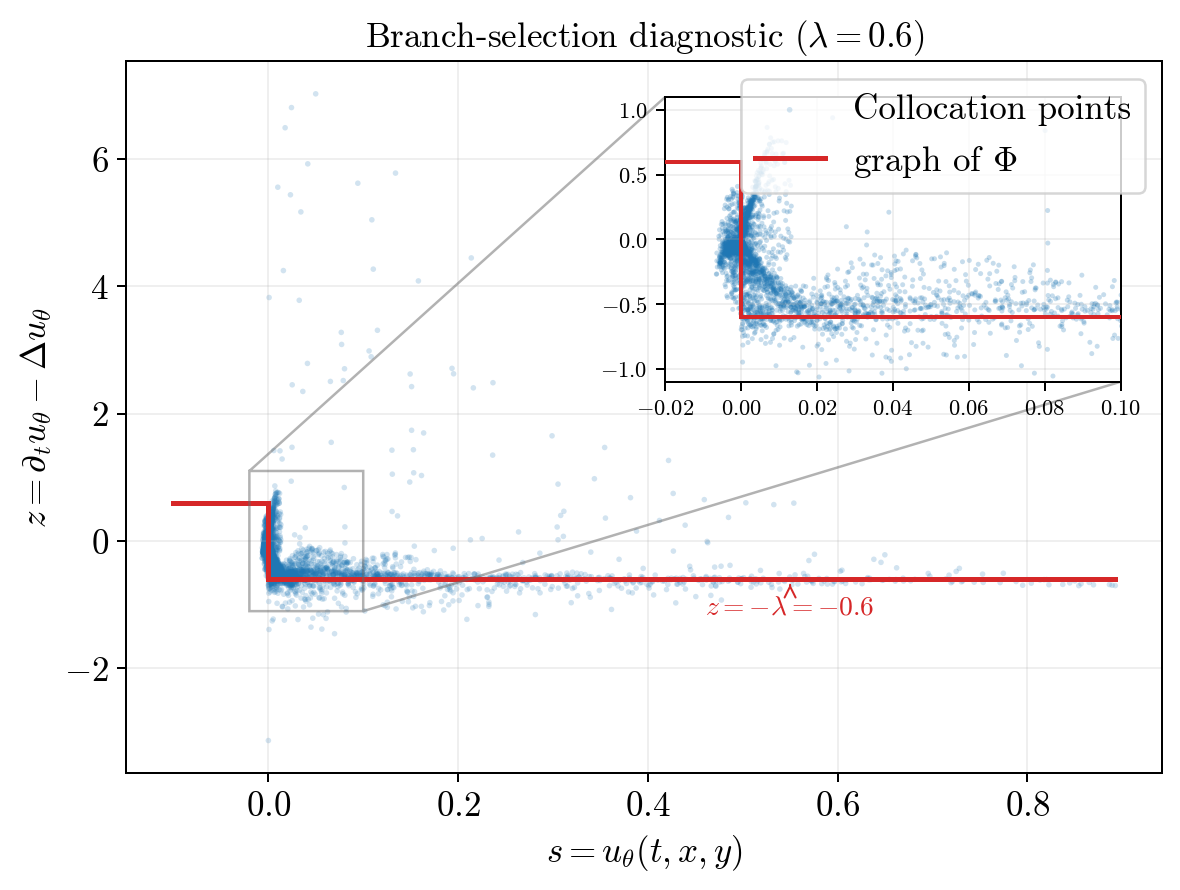
\includegraphics[width=0.72\textwidth]{figures/branch_selection_diagnostic.png}
  \caption{Branch-selection diagnostic ($\lambda=0.6$): empirical cloud of
    $(u_\theta,\,\partial_tu_\theta-\Delta u_\theta)$ at $4\,000$ post-training
    collocation points (blue dots), overlaid on the graph of $\Phi$ (red).
    Points with $s\gtrsim0.05$ cluster tightly on the branch $z=-0.6$;
    no points appear with $s<0$ (sign preservation by the relay flow);
    the vertical scatter near $s\approx0$ traces the extinction front,
    where the discontinuity of $\Phi$ limits pointwise accuracy. The inset
    magnifies the neighborhood of the extinction front ($s$ close to $0$).}
  \label{fig:relay-branch}
\end{figure}

Figure~\ref{fig:relay-sweep} and Table~\ref{tab:relay-extinction} summarize
the extinction-time comparison across the primary sweep
$\lambda\in\{0.4,0.6,0.8\}$. The DR-PINN norm curves reproduce the
qualitative shape of the reference curves for all three values of $\lambda$,
and the detected extinction times follow the correct ordering
$t^*(0.4)>t^*(0.6)>t^*(0.8)$. The absolute errors range from $0.006$ to
$0.012$ time units, growing modestly with $\lambda$; this is consistent with
the observation that the effective loss scale grows as $\lambda^2$ (the
distance-residual target $z\to\pm\lambda$ grows with $\lambda$), so that a
fixed training budget resolves the extinction front with slightly lower
absolute accuracy at larger $\lambda$.

\begin{figure}[htbp]
  \centering
  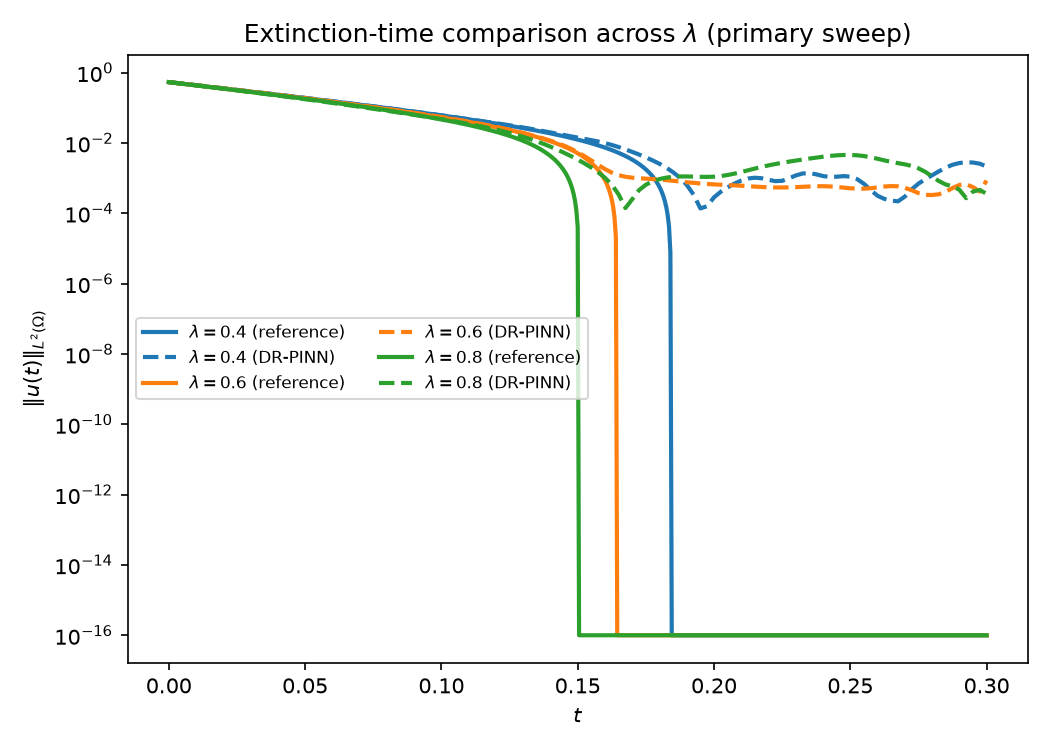
\includegraphics[width=0.80\textwidth]{figures/extinction_time_sweep.png}
  \caption{Extinction-time comparison across the primary sweep
    $\lambda\in\{0.4,0.6,0.8\}$. Solid lines: reference solver. Dashed lines:
    DR-PINN. Colors identify the three $\lambda$ values (blue: $0.4$, orange:
    $0.6$, green: $0.8$). Curves are clipped below $10^{-6}$ for readability:
    after extinction the reference drops to exactly zero (below the axis)
    while the DR-PINN norm stabilizes at $\approx10^{-4}$; the correct
    monotone ordering of extinction times is reproduced by the DR-PINN for all
    three values.}
  \label{fig:relay-sweep}
\end{figure}


%% ============================================================
\section{Conclusions}
\label{sec:conclusions}
%% ============================================================

\textcolor{red}{[Conclusions to be added here.]}



%% ============================================================
%%  References
%% ============================================================
%\bibliographystyle{amsplain} % Sorted alphabetically
\bibliographystyle{elsarticle-num} % Sorted by appearance in the text
\bibliography{references}

\end{document}
